%# -*- coding: utf-8-unix -*-
%%==================================================
%% thesis.tex
%%==================================================

\newcommand{\bs}{\boldsymbol}
\newcommand{\bd}{\bm{d}}
\newcommand{\bx}{\bs{x}}
\newcommand{\by}{\bs{y}}
\newcommand{\bz}{\bs{z}}
\newcommand{\br}{\bs{r}}
\newcommand{\bbm}{\bs{m}}
\newcommand{\bh}{\bs{h}}
\newcommand{\btheta}{\bs{\theta}}
\newcommand{\bw}{\bm{w}}
\newcommand{\bb}{\bs{b}}
\newcommand{\bS}{\bs{S}}
\newcommand{\score}{{SCoRe}}
\newcommand{\mg}{\bm{G}}
\newcommand{\argmin}{arg\,min}

\newcommand{\weinan}[1]{{\bf \color{blue} [[Weinan says ``#1'']]}}
\newcommand{\kan}[1]{{\bf \color{red} [[Kan says ``#1'']]}}
\newcommand{\jiarui}[1]{{\bf \color{green} [[Jiarui says ``#1'']]}}
\newcommand{\jian}[1]{{\bf \color{orange} [[Jian says ``#1'']]}}


% 双面打印
% \documentclass[doctor, openright, twoside]{sjtuthesis}
\documentclass[bachelor, openany, oneside, english, submit]{sjtuthesis}
% \documentclass[master, review]{sjtuthesis}
% \documentclass[%
%   bachelor|master|doctor|coursepaper, % 必选项,分别是学士,硕士,博士学位论文以及课程论文
%   fontset=fandol|windows|mac|ubuntu|adobe|founder, % 字体选项
%   oneside|twoside,        % 单面打印,双面打印(奇偶页交换页边距,默认)
%   openany|openright,      % 可以在奇数或者偶数页开新章|只在奇数页开新章(默认)
%   english,                % 启用英文模版
%   review,     % 盲审论文,隐去作者姓名、学号、导师姓名、致谢、发表论文和参与的项目
%   submit      % 定稿提交的论文,插入签名扫描版的原创性声明、授权声明
% ]

% 逐个导入参考文献数据库
\addbibresource{bib/thesis.bib}
% \addbibresource{bib/chap2.bib}

%# -*- coding: utf-8-unix -*-
% !TEX program = xelatex
% !TEX root = ../thesis.tex
% !TEX encoding = UTF-8 Unicode
%TC:ignore
\title{Collaborative Recommendation based on \\~Incremental Graph Learning}
\author{秦佳锐}
\advisor{张伟楠}
% \coadvisor{某某教授}
\defenddate{2014年12月17日}
\coursename{某某课程}
\school{上海交通大学}
\institute{电子信息与电气工程学院}
\studentnumber{515030910475}
% \cnacademicdegree{工学硕士}
\major{软件工程}
\keywords{协同过滤, 序列化推荐, 图注意力网络, 双序列建模}

\englishtitle{Collaborative Recommendation based on Incremental Graph Learning}
\englishauthor{\textsc{Mo Mo}}
\englishadvisor{Prof. \textsc{Mou Mou}}
% \englishcoadvisor{Prof. \textsc{Uom Uom}}
\englishschool{Shanghai Jiao Tong University}
\englishinstitute{\textsc{Depart of XXX, School of XXX} \\
  \textsc{Shanghai Jiao Tong University} \\
  \textsc{Shanghai, P.R.China}}
\englishinstitutemaster{Depart of XXX, \\ School of XXX}
\englishmajor{A Very Important Major}
\englishdate{Dec. 17th, 2014}
\enacademicdegree{Master of Engineering}
\englishstudentid{0010900990}
\englishkeywords{Collaborative Filtering, Sequential Recommendation, Graph Attention Network, Dual Sequences Modeling}
%TC:endignore
  % NOTE: the enclosed commands must be executed in preamble

\begin{document}

% 无编号内容:中英文论文封面、授权页
\maketitle
\makeatletter

\ifsjtu@coursepaper
% 摘要 部分课程论文需要,可以自行选择添加或者去除
% %# -*- coding: utf-8-unix -*-
% !TEX program = xelatex
% !TEX root = ../thesis.tex
% !TEX encoding = UTF-8 Unicode
%%==================================================
%% abstract.tex for SJTU Master Thesis
%%==================================================

\begin{abstract}
推荐系统 (Recommendation Systems)是一类信息过滤系统,它解决用户在商用系统中信息过载的问题,
目前推荐系统越来越成为互联网世界重要的组成部分。推荐系统的核心任务是预测用户对某件商品的喜好。
目前推荐系统邻域最流行的算法是协同过滤算法 (Collaborative Filtering),它一般通过矩阵分解
的方法学习用户/商品的隐变量,并且希望能够对用户间/商品间的相似关系进行建模。但是,协同过滤
忽略了用户兴趣与商品性质随时间变化的动态过程,而且它只利用用户自己交互过的商品 (或商品自己交互过的用户) 信息
去反映用户的兴趣 (商品的性质)。
有一些工作提出了一些捕捉用户兴趣随时间变化的方法,但是这些方法
只考虑用户端的行为序列,而忽视了商品端的时间序列变化 (商品不同时刻吸引不同的用户)。并且这些序列
建模的方法忽视了协同关系,比如不同用户间的相似兴趣、商品间的相似性质等。
在本篇文章中,我们从时序增量图的视角出发,提出了一种结合协同过滤与序列模型的方法: \textbf{S}equential \textbf{Co}llaborative \textbf{Re}commender 
(\score),它从时间和空间两个维度出发,不仅在时间维度上同时建模用户和商品的两段序列,也在空间
维度上建模用户间 (商品间)的协同关系,从而达到更好的建模效果。通过在三个大规模真实世界数据集上的实验,
我们提出的模型相比目前有的方法有着明显的提高。


\end{abstract}

\begin{englishabstract}
    Recommender system alleviates information overload for the users on online business platforms, thus it has become a key part in online information systems. The core task of recommender system is to predict the user preference over the items.
    The most widely adopted methodology is collaborative filtering implemented through factorization models or latent factor-based models, which seeks to utilize the similarity among users or items. However, it ignores the temporal dynamics such as the changing preference of the user and popularity trends of the item, and it only uses target user's (or item's) own interacted items (users) to indicate user interests (or item attractions).
    Several works have been proposed to capture sequential patterns of the user's interests, while they do not consider the item-side temporal dynamics. Worse still, the dynamics of collaborative relations, i.e., similar tastes of users or analogous properties of items at different time, have been abandoned in these sequential recommendation models. 
    In this paper, we take an intersectional view and propose \textbf{S}equential \textbf{Co}llaborative \textbf{Re}commender (\score) which not only captures the \textit{temporal} patterns from both user-side and item-side behavior sequences, but also collaboratively synthesizes the \textit{spatial} information from user-item interaction graph at each time slice for better modeling. The comprehensive experiments over three real-world large-scale datasets show the significant improvement of the proposed model.

\end{englishabstract}



% 目录 部分课程论文需要,可以自行选择添加或者去除
% \tableofcontents

\else
  \ifsjtu@submit\relax
    % 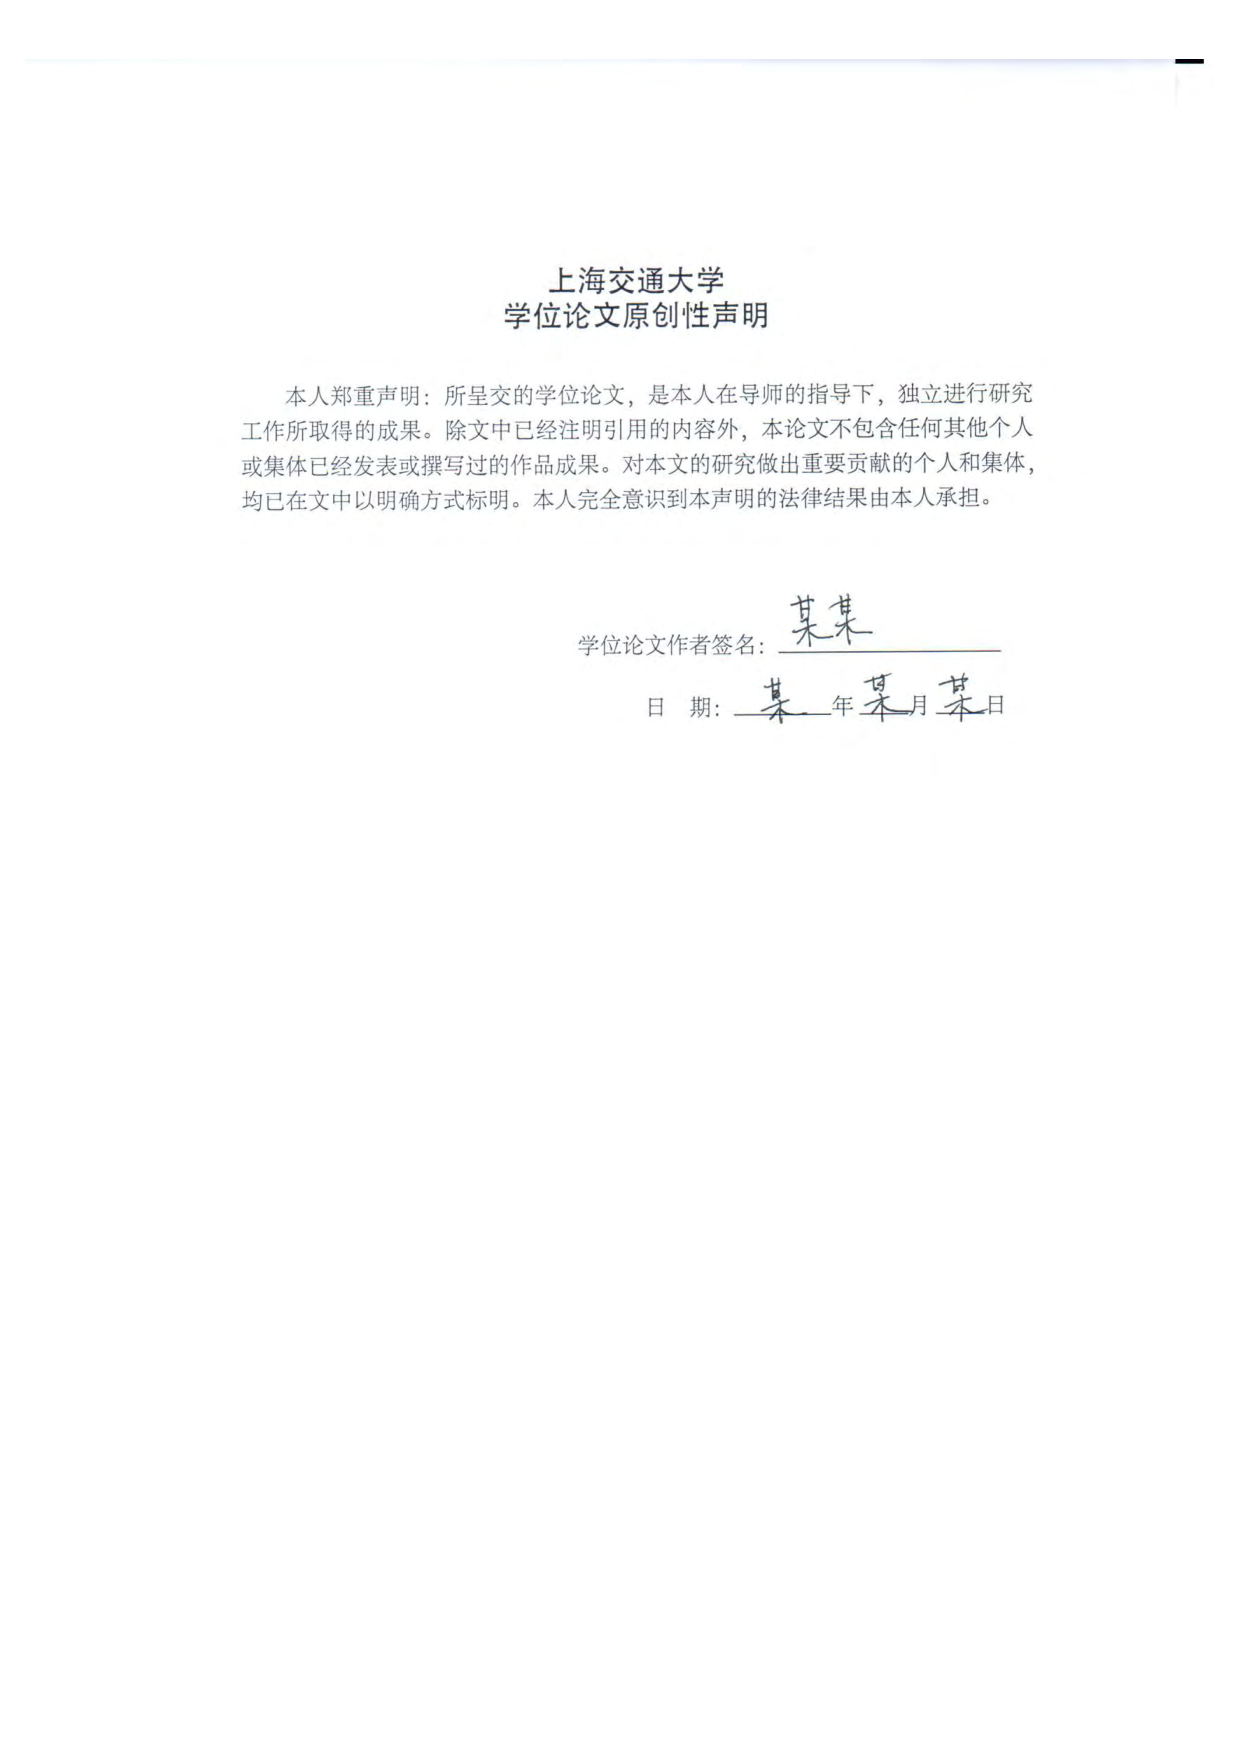
\includepdf{pdf/original.pdf}
    \cleardoublepage
    % 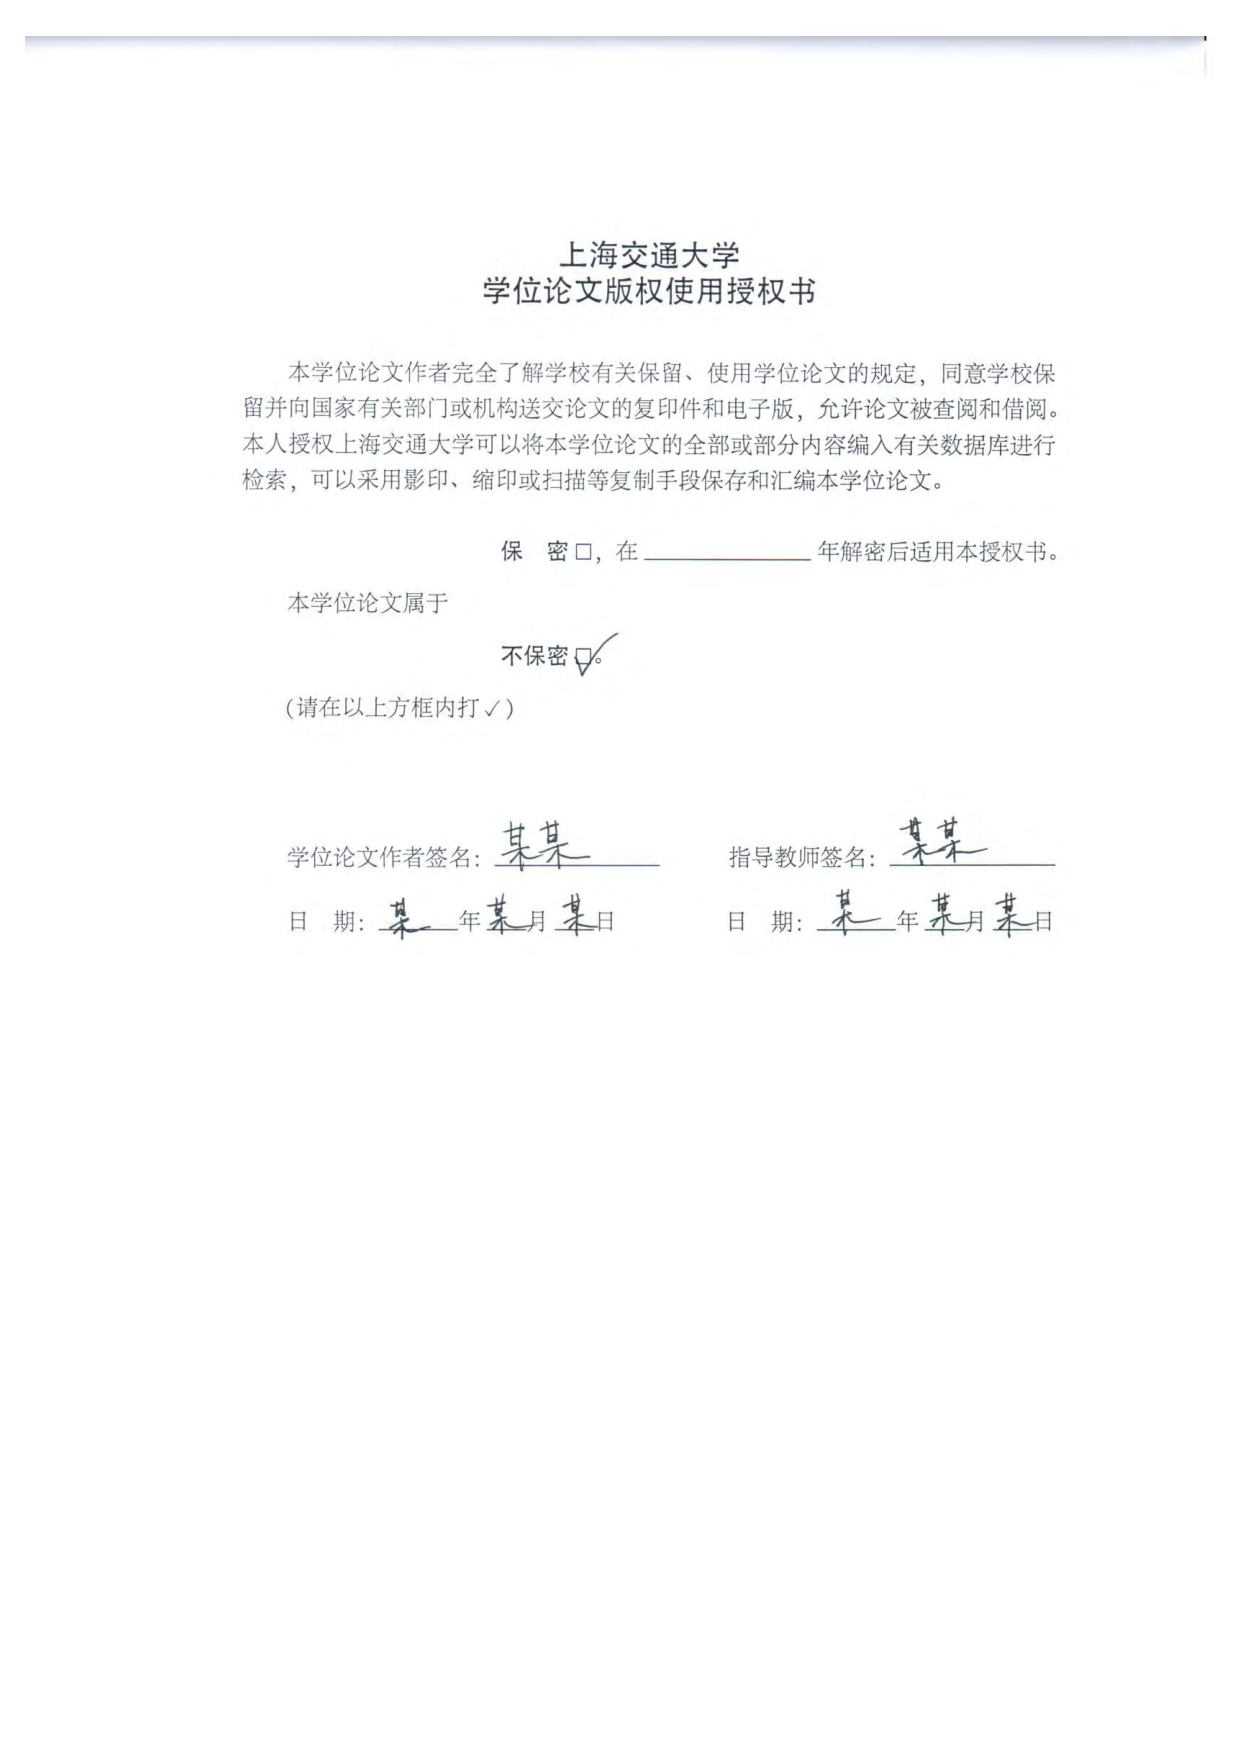
\includepdf{pdf/authorization.pdf}
    \cleardoublepage
  \else
    \ifsjtu@review\relax
    % exclude the original claim and authorization
    \else
      \makeDeclareOriginal
      \makeDeclareAuthorization
    \fi
  \fi
  \frontmatter % 使用罗马数字对前言编号

  % 摘要
  %# -*- coding: utf-8-unix -*-
% !TEX program = xelatex
% !TEX root = ../thesis.tex
% !TEX encoding = UTF-8 Unicode
%%==================================================
%% abstract.tex for SJTU Master Thesis
%%==================================================

\begin{abstract}
推荐系统 (Recommendation Systems)是一类信息过滤系统,它解决用户在商用系统中信息过载的问题,
目前推荐系统越来越成为互联网世界重要的组成部分。推荐系统的核心任务是预测用户对某件商品的喜好。
目前推荐系统邻域最流行的算法是协同过滤算法 (Collaborative Filtering),它一般通过矩阵分解
的方法学习用户/商品的隐变量,并且希望能够对用户间/商品间的相似关系进行建模。但是,协同过滤
忽略了用户兴趣与商品性质随时间变化的动态过程,而且它只利用用户自己交互过的商品 (或商品自己交互过的用户) 信息
去反映用户的兴趣 (商品的性质)。
有一些工作提出了一些捕捉用户兴趣随时间变化的方法,但是这些方法
只考虑用户端的行为序列,而忽视了商品端的时间序列变化 (商品不同时刻吸引不同的用户)。并且这些序列
建模的方法忽视了协同关系,比如不同用户间的相似兴趣、商品间的相似性质等。
在本篇文章中,我们从时序增量图的视角出发,提出了一种结合协同过滤与序列模型的方法: \textbf{S}equential \textbf{Co}llaborative \textbf{Re}commender 
(\score),它从时间和空间两个维度出发,不仅在时间维度上同时建模用户和商品的两段序列,也在空间
维度上建模用户间 (商品间)的协同关系,从而达到更好的建模效果。通过在三个大规模真实世界数据集上的实验,
我们提出的模型相比目前有的方法有着明显的提高。


\end{abstract}

\begin{englishabstract}
    Recommender system alleviates information overload for the users on online business platforms, thus it has become a key part in online information systems. The core task of recommender system is to predict the user preference over the items.
    The most widely adopted methodology is collaborative filtering implemented through factorization models or latent factor-based models, which seeks to utilize the similarity among users or items. However, it ignores the temporal dynamics such as the changing preference of the user and popularity trends of the item, and it only uses target user's (or item's) own interacted items (users) to indicate user interests (or item attractions).
    Several works have been proposed to capture sequential patterns of the user's interests, while they do not consider the item-side temporal dynamics. Worse still, the dynamics of collaborative relations, i.e., similar tastes of users or analogous properties of items at different time, have been abandoned in these sequential recommendation models. 
    In this paper, we take an intersectional view and propose \textbf{S}equential \textbf{Co}llaborative \textbf{Re}commender (\score) which not only captures the \textit{temporal} patterns from both user-side and item-side behavior sequences, but also collaboratively synthesizes the \textit{spatial} information from user-item interaction graph at each time slice for better modeling. The comprehensive experiments over three real-world large-scale datasets show the significant improvement of the proposed model.

\end{englishabstract}



  % 目录、插图目录、表格目录
  \tableofcontents
  \listoffigures
  \addcontentsline{toc}{chapter}{\listfigurename}     % 将插图目录加入全文目录
  \listoftables
  \addcontentsline{toc}{chapter}{\listtablename}      % 将表格目录加入全文目录
  % \listofalgorithms
  % \addcontentsline{toc}{chapter}{\listalgorithmname}  % 将算法目录加入全文目录

  % %# -*- coding: utf-8-unix -*-
% !TEX program = xelatex
% !TEX root = ../thesis.tex
% !TEX encoding = UTF-8 Unicode
%TC:ignore
\begin{nomenclaturename}
\label{chap:symb}

\begin{longtable}{rl}
$\epsilon$     & 介电常数 \\
 $\mu$ 		& 磁导率 \\
 $\epsilon$     & 介电常数 \\
 $\mu$ 		& 磁导率 \\
 $\epsilon$     & 介电常数 \\
 $\mu$ 		& 磁导率 \\
 $\epsilon$ 	& 介电常数 \\
 $\mu$ 		& 磁导率 \\
 $\epsilon$     & 介电常数 \\
 $\mu$ 		& 磁导率 \\
 $\epsilon$     & 介电常数 \\
 $\mu$ 		& 磁导率 \\
 $\epsilon$     & 介电常数 \\
 $\mu$ 		& 磁导率 \\
 $\epsilon$ 	& 介电常数 \\
 $\mu$ 		& 磁导率 \\
 $\epsilon$     & 介电常数 \\
 $\mu$ 		& 磁导率 \\
 $\epsilon$     & 介电常数 \\
 $\mu$ 		& 磁导率 \\
 $\epsilon$     & 介电常数 \\
 $\mu$ 		& 磁导率 \\
 $\epsilon$ 	& 介电常数 \\
 $\mu$ 		& 磁导率 \\
 $\epsilon$     & 介电常数 \\
 $\mu$ 		& 磁导率 \\
 $\epsilon$     & 介电常数 \\
 $\mu$ 		& 磁导率 \\
 $\epsilon$     & 介电常数 \\
 $\mu$ 		& 磁导率 \\
 $\epsilon$ 	& 介电常数 \\
 $\mu$ 		& 磁导率 \\
 $\epsilon$     & 介电常数 \\
 $\mu$ 		& 磁导率 \\
 $\epsilon$     & 介电常数 \\
 $\mu$ 		& 磁导率 \\
 $\epsilon$     & 介电常数 \\
 $\mu$ 		& 磁导率 \\
 $\epsilon$ 	& 介电常数 \\
 $\mu$ 		& 磁导率 \\
 $\epsilon$     & 介电常数 \\
 $\mu$ 		& 磁导率 \\
 $\epsilon$     & 介电常数 \\
 $\mu$ 		& 磁导率 \\
 $\epsilon$     & 介电常数 \\
 $\mu$ 		& 磁导率 \\
 $\epsilon$ 	& 介电常数 \\
 $\mu$ 		& 磁导率 \\
 $\epsilon$     & 介电常数 \\
 $\mu$ 		& 磁导率 \\
 $\epsilon$     & 介电常数 \\
 $\mu$ 		& 磁导率 \\
 $\epsilon$     & 介电常数 \\
 $\mu$ 		& 磁导率 \\
\end{longtable}

\end{nomenclaturename}
%TC:endignore
 % 主要符号、缩略词对照表
\fi

\makeatother
\mainmatter % 使用阿拉伯数字对正文编号

% 正文内容
%# -*- coding: utf-8-unix -*-
% !TEX program = xelatex
% !TEX root = ../thesis.tex
% !TEX encoding = UTF-8 Unicode
%%==================================================
%% chapter01.tex for SJTU Master Thesis
%%==================================================

%\bibliographystyle{sjtu2}%[此处用于每章都生产参考文献]

\chapter{Introduction}
\label{sec:intro}
Nowadays, recommender systems have been widely used in most Internet-based services, such as news feeds \cite{wang2017dynamic,liu2010personalized} and e-commerce platform \cite{rendle2010factorizing}.
The goal of recommender system is to select the items or contents that the target user tends to like, which alleviates the information overload in a large margin \cite{zhang2017deep} of online information systems.

The researchers in both academic and industrial fields have devoted many efforts on this research hotspot.
Among the existing methods, the most widely adopted solution is based on collaborative filtering originating from \cite{goldberg1992using}.
It achieves the goal of recommendation through learning only from historical user-item interactions, either explicit (i.e., user ratings over items) or implicit (i.e., user clicks) feedbacks \cite{zhang2017deep} without exogenous information about items or users.
The collaborative filtering (CF) methodologies seek to capture the collaborative relations among different users with similar tastes \cite{koren2008factorization} to provide recommendations to the target user.

% spatial information: user-item interactions
%\kan{need an illustration of user-item interaction graph to represent first-order interactions of the target item and the target user.}
\begin{figure}[h]
	\centering
	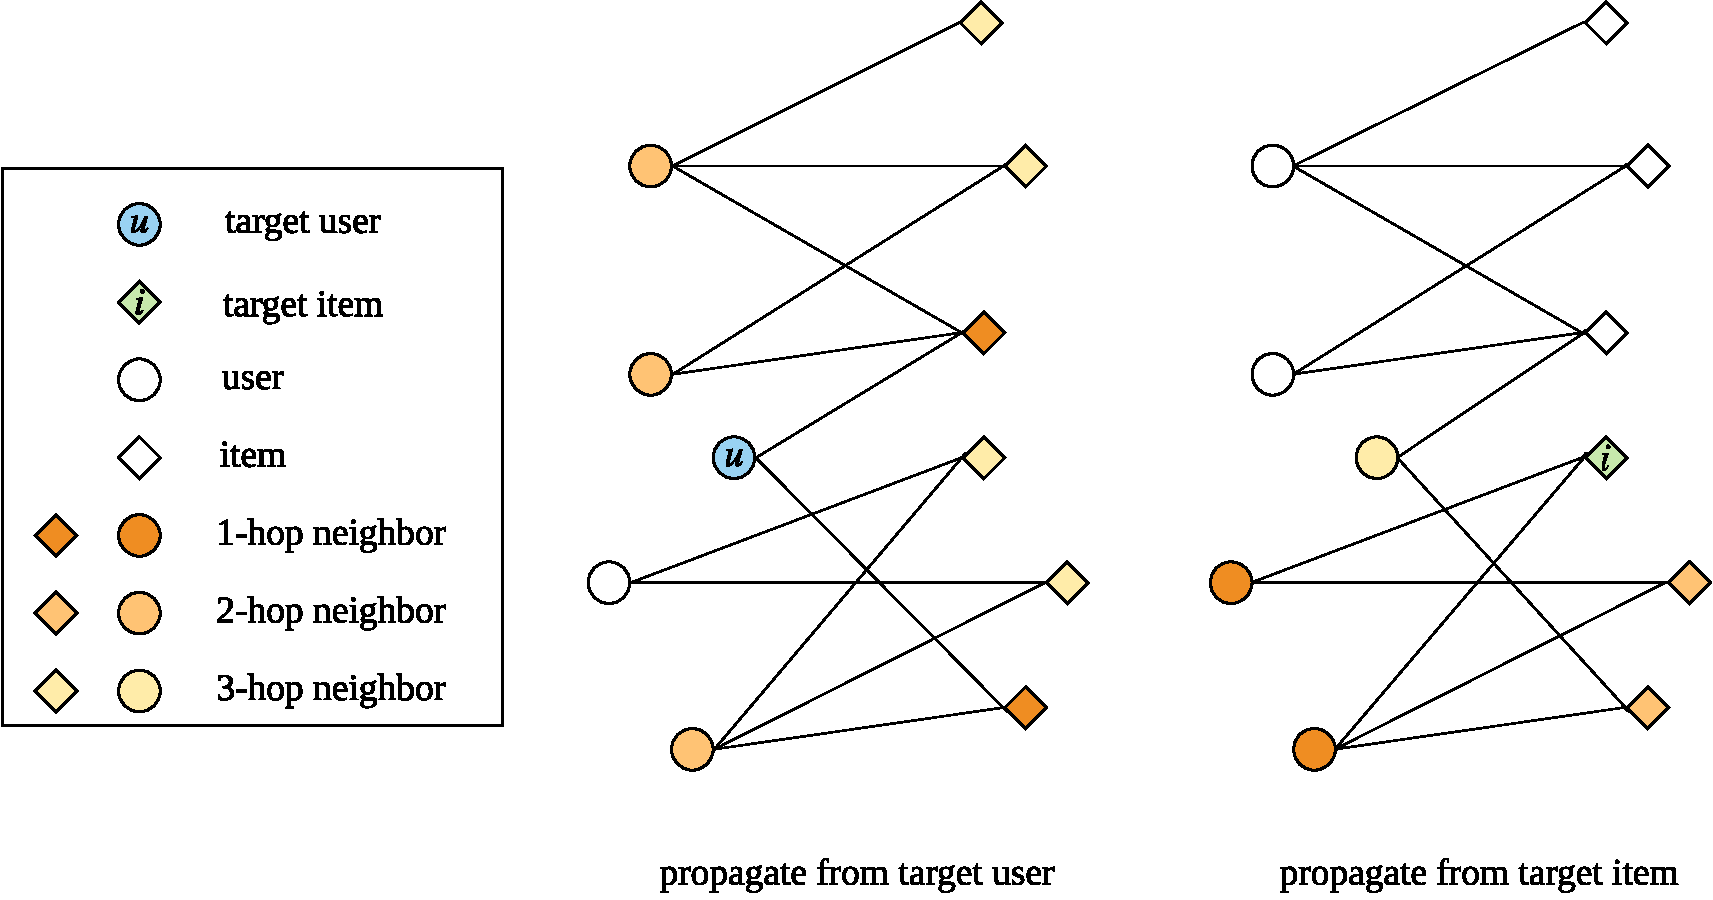
\includegraphics[width=1.0\columnwidth]{intro.pdf}
	\caption{Graph illustration of target user/item-rooted subgraph.}
	\label{fig:bi-graph}
\end{figure}
% Some methods \cite{niu2018collaborative,talasu2017link,ying2018graph,fadel2018link,van2017graph,wu2019session} regard the recommendation task as a link prediction problem with the consideration of the existing node connections (user-item interactions), as is shown in Figure~\ref{fig:bi-graph}.
% The view of traditional collaborative filtering is a first-order graph pattern mining since the interactions between the target user and the visited items conduct the first-order connections from the user in the bipartite graph of user-item interactions.
% Nevertheless, these methodologies only regard the feature extraction for the target user (or the target item) as neighborhood gathering \cite{kipf2016semi}, which does not incorporate the collaborative influence among the gathered nodes \kan{to refine; to add collaborative relations.}, as shown by the dotted line in Figure~\ref{fig:bi-graph}. \jiarui{refine figure 1 or sentence}
% Moreover, they consider the related interactions in the bipartite graph to the target, while ignoring the temporal patterns for the evolving graph of user-item interactions.
Some methods \cite{niu2018collaborative,talasu2017link,ying2018graph,fadel2018link,van2017graph,wu2019session} regard the recommendation task as a link prediction problem, which is to predict the probability of link relation, e.g., clicks and conversions, between the target user and the target item.
They consider the existing node connections (user-item interactions) as the feature for link prediction.
The view of traditional CF is a first-order graph pattern mining since the interactions between the target user and the visited items conduct the first-order connections in the user-item bipartite graph as is shown in Fig.~\ref{fig:bi-graph}. 
%\kan{it seems that kth-order means ``to predict k links'', but we only use k links as features. it should needs confirmation.}
These methodologies only use the first-order neighbors through one-hop propagation to represent the target user (or target item) and learn the representations of users/items though reconstructing the rating matrix.
These models utilize the "collaborative" information in an implicit way by learning the representation of users and items. However, they ignore the collaborative information that can be found by propagating over the user-item bipartite graph.
That is to find the users who share the same interests  (interacted with same group of items) with the target user.
These users from this subgraph can be used to enhance the representation of the target user. And it can be done in a similar way from the side of the target item. The propagation process over the subgraph can be conducted many times as shown in Fig~\ref{fig:bi-graph}.

% another con is the ignorance of collaborative relations

% temporal dynamics 
As has been stated in many related works \cite{hidasi2017recurrent,koren2009collaborative,he2016vista,agarwal2009spatio}, the temporal dynamics have high impacts on future user behaviors, especially accounted for concept drifting \cite{widmer1996learning}, long-term behavior dependency \cite{koren2009collaborative}, periodic patterns \cite{ren2018repeatnet}, etc.
However, most CF models regard the user-item bipartite graph as a static entirety while ignoring the temporal dynamics of user-item interactions.
Yet some other researchers tend to utilize state-based methods \cite{he2016fusing,he2016vista} or sequential modeling \cite{hidasi2017recurrent,tang2018personalized,ren2019lifelong} to capture the dynamic user behavior patterns, especially for sequential recommendation \cite{huang2018improving,chen2018sequential,kang2018self,tang2018personalized} problem.
There are two drawbacks hidden in the existing sequential modeling works.
The one is that they only consider the changing preference of the user, while the temporal dynamics of the item have been abandoned.
For example, the popularity of the existing item may change over time \cite{koren2009collaborative} according to some factors such as gloves are more popular in winter than in summer; and some products may involve sales promotion in some time to attract new group of users. %Such that people may show preference to different items at different time even though their tastes remain the same during that period.
%The other con is that few of them utilize the spatial information of the graph for the sequential modeling at each time, thus lacking of global pattern mining.
Such that the same item may attract different users at different time even though its properties are stable along the time.
The other con is that few of them utilize the collaborative information provided by similar users or similar items. These sequential recommendation models tend to only memorize the target user's own interest dynamics while they lack of a wider range of considerations.
% collaborative filtering and sequential recommendation
% drawbacks


Generally speaking, the \textit{spatial} collaborative graph information and the \textit{temporal} sequential patterns both influence the final recommendation.
To comprehensively utilize the spatial-temporal information with collaborative filtering, we propose \textbf{S}equential \textbf{Co}llaborative \textbf{Re}commender (\score).
The model firstly conducts the incremental subgraphs originating from the target user and the target item along time.
Secondly, it fully utilizes the spatial information given by the local subgraph through mining the collaborative patterns with multi-hop propagation over graph neighbors.
%by mining the patterns through multiple hop propagation over graph 
Finally, it also captures the sequential patterns along the evolving user-item graph from both sides of the target user and the target item.%and finally adopts collaborative filtering for the subgraphs at each time slice for better modeling the evolving graph patterns of user (item) similarities.

Specifically, for user-item interaction graph at each time slice, we utilize the proposed \textit{Co-Attention Graph Network} to aggregate the spatial information gathered by multi-hop propagation in a collaborative manner.
Then we apply a non-linear recurrent neural network (RNN) for modeling the temporal patterns of the evolving graph, with the consideration of the obtained collaborative relations.
By this way, our model has the knowledge of (i) which group of people would share the similar tastes at each time (through multi-hop propagation on the graph), (ii) how their preferences evolve along the timeline (through non-linear recurrent model).
Moreover, not just modeling the user behaviors, \score~ can also consider from the item side and well capture the item trends for better user-item matching in the final recommendation by utilizing an interactive attention mechanism.
For example, this recommender system may present Christmas card to a user when the holiday is coming even \textit{before} her interacting with any related items. This goal would be obtained by using the interests of similar users to her and model the temporal dynamics properly.

% advantage
% a new perspective for recommender system with spatial-temporal pattern mining
% non-linear temporal pattern mining and collaborative relation discovery through co-attention mechanism
% dynamic system for varying user preferences and diversified trends of items
To the best of our knowledge, this is the first work which models the sequential recommendation task as incremental graph learning problem. It applies unified spatial-temporal graph pattern mining with collaborative filtering for the recommender systems.
The contribution of the paper lies in three-fold:
\begin{itemize}[leftmargin=5mm]
	\item \textbf{Spatial and Temporal Graph Pattern Mining.} We slice the user-item interactions as a series of evolving bipartite graph along the timeline, and propose a comprehensive framework with spatial-temporal pattern mining for final recommendation.
	\item \textbf{Dual Sequence Modeling.} We apply the spatial and temporal pattern mining from both sides of user and item, which derives a comprehensive modeling result.
%	 \textit{Co-Attention Graph Network} to aggregate multiple hops information on the user-item interaction graph in a collaborative manner.
%	\item \textbf{Temporal Graph Pattern Mining}: We propose \textit{Interactive Attention Mechanism} to model the problem of link prediction (between the target user and target item) for the dynamic incremental graphs. We use subgraph sequences from both target user's and target item's side.
	\item \textbf{State-of-the-art Performance.} We evaluate and compare our model with several strong baselines over three real-world and large-scale recommendation datasets. The results have proven the efficacy of \score ~model.
\end{itemize}

The rest of the paper is scheduled as below.
In Section~\ref{sec:rel}, we discuss about some related works.
Section~\ref{sec:method} presents the \score~model in detail and we also make some discussion about the relatedness to the existing works.
We conduct some comprehensive experiments and present the experimental setups with the corresponding results in Section~\ref{sec:exps}.
Finally we conclude the paper and point out some future works in Section~\ref{sec:con}.

\chapter{Related Work}\label{sec:rel}

\section{Recommender Systems}
With the rapid development of the Internet and the widespread use of large data
storage and processing systems, it is very easy to access large volumn data today.
However, it is more and more diffcult to find the really related, interesting and 
useful data which is called \textit{information overload}.

Over the last few decades, there has been a significant amount of research on 
computer applications that can discover tailored appropriate content. Among these
research, search engines and recommender systems are the two main methodologies.

Both recommender systems and search engines aim to alleviate the information overload
problem, however in different manner. For search engines, the user's intentions are
clear which are indicated by the search keywords, while for the recommender systems,
the user's intentions are vague. Users just hanging in the Internet without a specific
intention. So, recommender system needs to recommend items to the users in this situation.

Furthermore, with the development of the Internet applications, recommender systems are
supposed to provide personal recommendation to the users, which means different
users should be recommended with different items, and these items should satisfy the
users' interests.

For a typical recommender system, the recommendation problem can be splitted into 
two folds: (i) prediction process. Estimating prediction for a single item; 
(ii) ranking process. Ranking the items according to the prediction value in 
the former step. While the former process is triggered by the user and 
focuses on predicting the probability of the user will like the item in 
question, the latter process is provided by the recommendation system itself 
and offers an ordered top-N list of items that the user might like.

There are three main categories of recommender systems:
\begin{itemize}
    \item \textit{CF recommender} produces recommendation based on other users
        with similar tastes and interests. 
    \item \textit{Content-based recommender} provides recommendation based on 
        the similarity between items and exploiting the descriptive characteristics of
        items which are liked by the users.
    \item \textit{Hybrid recommender} combines the former two ways and it overcomes
        the disadvantages of the other methods.
\end{itemize}

\section{Collaborative Filtering}
In recommender system literatures, the most widely used method is 
collaborative filtering \cite{goldberg1992using}, which learns from 
the historical user-item interactions without exogenous information 
about items or users. It recommends according to the modeled user 
preferences, e,g., clicks \cite{qu2016product,agarwal2009spatio} and 
ratings \cite{koren2009collaborative}, over the items.
As shown in Fig.~\ref{fig:cf}, in a recommender system, there are $m$ users, 
$\{u_1, u_2, ..., u_m\}$ and $n$ items, $\{p_1, p_2, ..., p_n\}$. The task is
to predict the rating of the active user $a$ on item $q$. Then rank the items 
according to the prediction rating, and forms the top-N items for user $a$.
CF models seek to learn dense vector representations of users and items, 
and predicts ratings using these representations. CF models represent a 
user by the items that she used to like/click. When every users are 
represented in this way, the similarity of users can be found and used.
\begin{figure}[h]
	\centering
	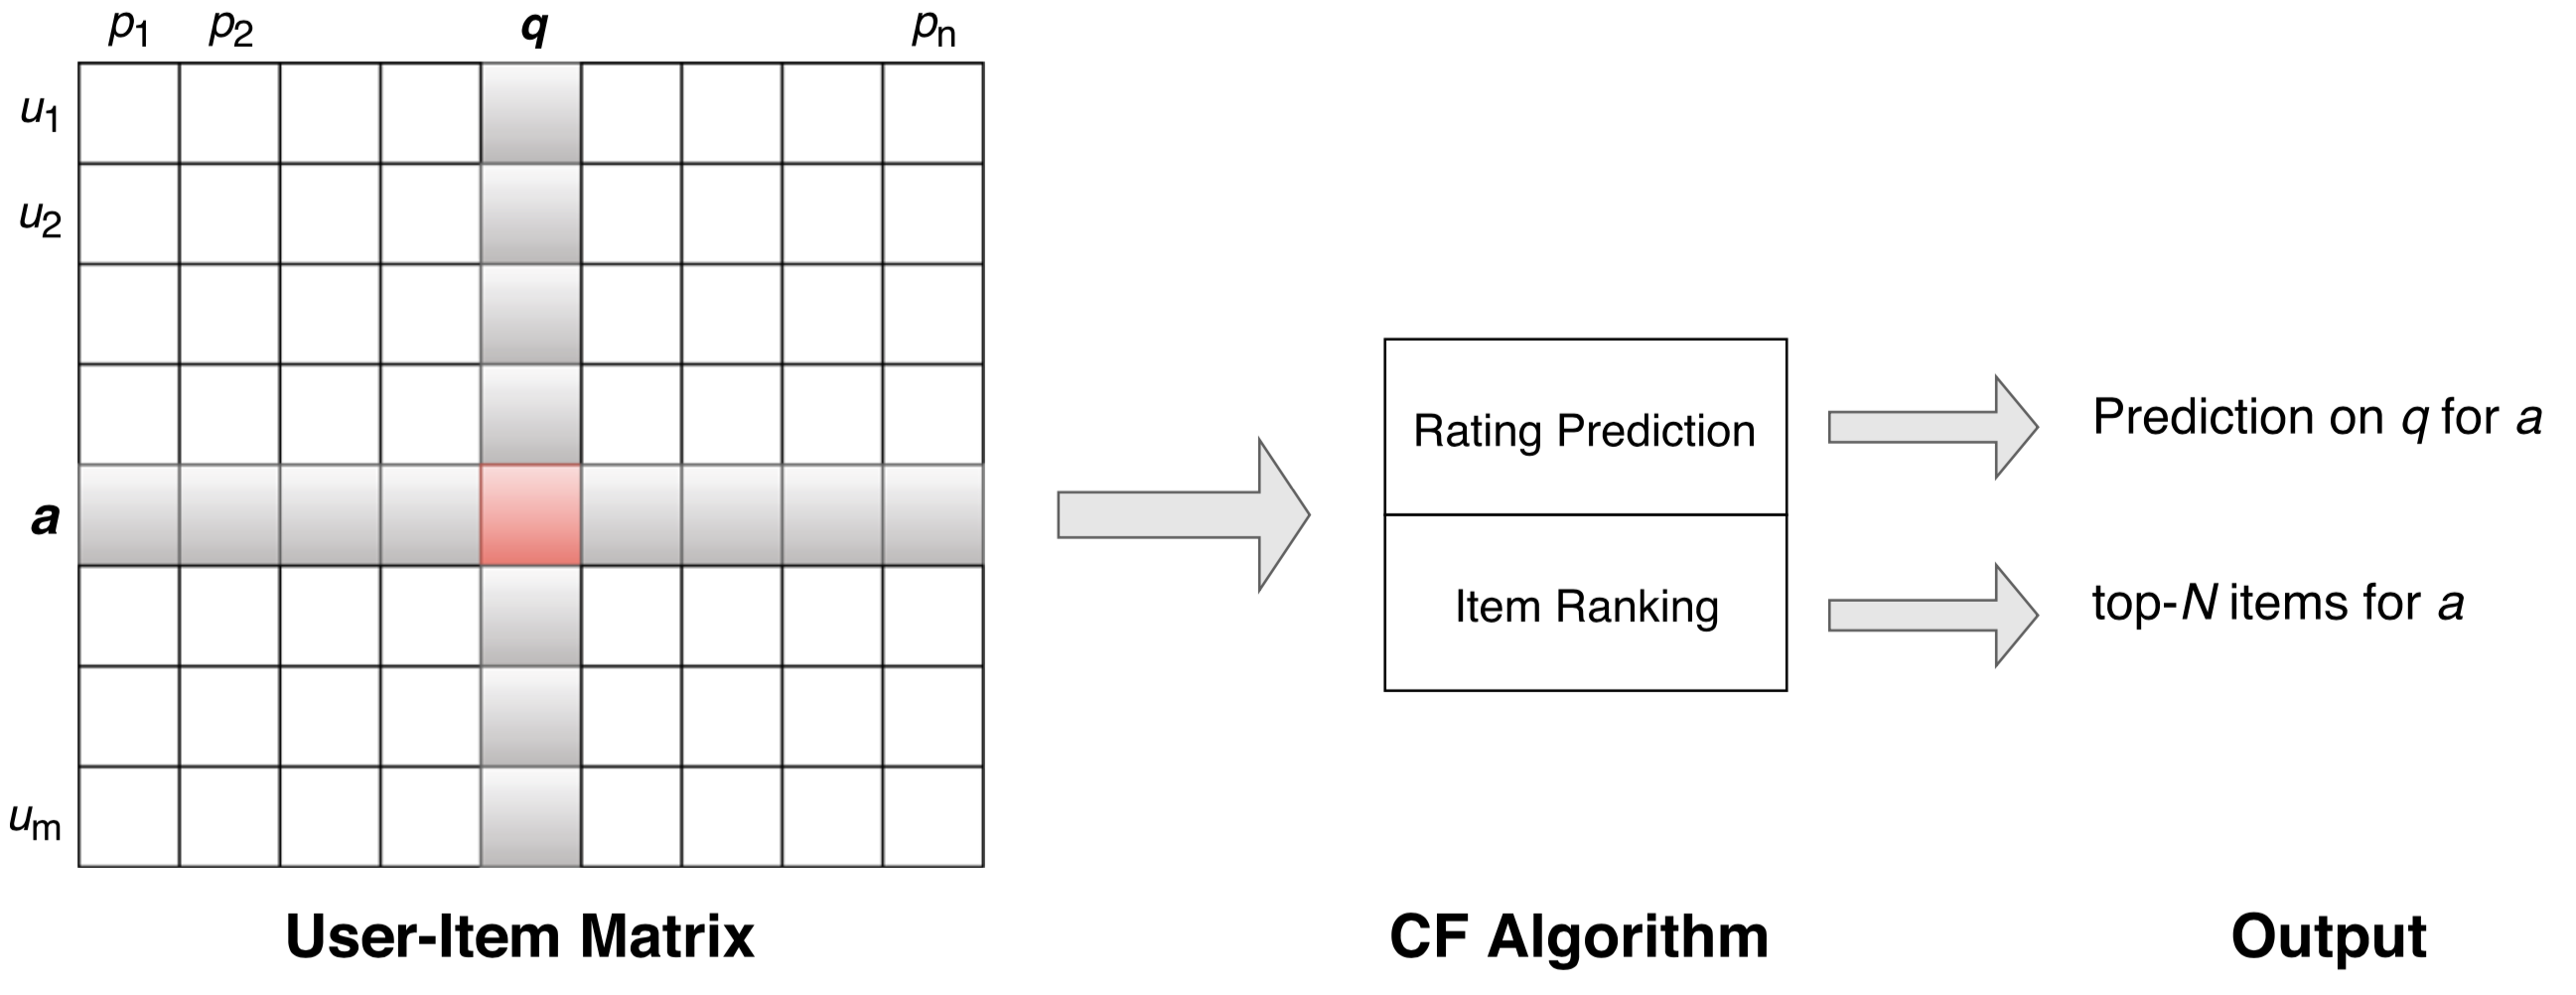
\includegraphics[width=0.9\columnwidth]{CF.png}
	\caption{An overview of the CF process.}
	\label{fig:cf}
	\vspace{-10pt}
\end{figure}
It is important that in such CF systems, preferences of like-minded neighbor 
users form the basis of all produced recommendations rather than individual 
features of items.

Many works \cite{koren2009matrix,salakhutdinov2007probabilistic,yang2012local,zhang2013optimizing} have been proposed based on collaborative filtering.
Among them, latent factor models play a key role in CF methods, ranging from pLSA \cite{hofmann2004latent} and Latent Dirichlet Allocation \cite{blei2003latent} to SVD-based models \cite{koren2008factorization,chen2012svdfeature} and factorization machines \cite{rendle2010factorization}.
% matrix factorization
% neural network for collaborative filtering
Nowadays, deep neural network (DNN) has attracted huge attentions in recommender systems because of its effective feature extraction and end-to-end model training with satisfying generalization \cite{zhang2017deep}.
Some DNN methods \cite{he2017neural,he2018outer,qu2016product} are proposed for latent factor collaborative filtering.
% temporal dynamics for CF-based model
However, almost all of these approaches, either conventional matrix factorization methods or deep models, lack of temporal pattern mining. And the ``collaborative'' part of these models are implicit, though latent factor representation learning.
\cite{koren2009collaborative} firstly proposed a SVD method for temporal dynamics while the model makes several assumptions with hand-engineered temporal bias thus it has poor generalization.
%\cite{wu2017recurrent} utilized RNN for sequence modeling. However, this work does not consider spatial graph information, and the model applis simple sum-pooling of the interacted items in each time slice thus not effective.

We will describe these models in detail in the following subsections:
\subsection{Latent Factor Models}
In this part, we take the famous SVD-based model as an example to describe
the latent factor models.
SVD models are actually a matrix factorization method which map both users 
and items to a joint latent factor space of a low dimention and ratings are
modeled as inner product in that space. Formally, each user $u$ is represented
by a dense vector $p_u \in R^d$ and each item is represented as $q_i \in R^d$
. The rating is calculated as $\hat{r_{ui}} = p_u^T q_i$. To learn the representations
of users and items, we minimize the regularized the squared error:
\begin{equation}
    \min _{q_{*}, p_{*}} \sum_{(u, i, t) \in \mathcal{K}}\left(r_{u i}-q_{i}^{T} p_{u}\right)^{2}+\lambda\left(\left\|q_{i}\right\|^{2}+\left\|p_{u}\right\|^{2}\right).
\end{equation}
This design is not good enough for much of the existed rating values 
are due to effects associated with either users or items, instead of 
their interactions. So bias terms for both user and item are needed in the model.
To achieve this, we use 
\begin{equation}
        \hat{r}_{u i}=\mu+b_{u}+b_{i}+q_{i}^{T} p_{u},
\end{equation}
to calculated the predicted ratings.
Koren et al\cite{koren2008factorization} extended the above model by adding the influence
of the user's interacted items as a feature to the prediction model, as
\begin{equation}
    \hat{r}_{u i}=\mu+b_{i}+b_{u}+q_{i}^{T}\left(p_{u}+|\mathrm{R}(u)|^{-\frac{1}{2}} \sum_{j \in \mathrm{R}(u)} y_{j}\right),
\end{equation}
where the set $R(u)$ contains the items that interacted with user $u$.


\subsection{DNN-based CF Models}
In this section, we present two works that are recently proposed for DNN-based
collaborative filtering recommender.

The first one is NCF \cite{he2017neural} which main contribution is replacing
the inner product with a neural architecture that can learn an arbitrary 
function from data. NCF is generic and can express and generalize matrix 
factorization under its framework.
The formulated framework of NCF is 
\begin{equation}
    \hat{y}_{u i}=f\left(\mathbf{P}^{T} \mathbf{v}_{u}^{U}, \mathbf{Q}^{T} \mathbf{v}_{i}^{I} | \mathbf{P}, \mathbf{Q}, \Theta_{f}\right)
\end{equation}
where $P \in R^{M \times K}$ and $P \in Q^{M \times K}$, denoting the 
latent factor matrix for users and items, respectively; and $\Theta_{f}$
is the parameters set of of the function $f$ which is implemented as a
neural network. Because $f$ is actually a multi-layer perceptron, the 
prediction function can be formulated as
\begin{equation}
    f\left(\mathbf{P}^{T} \mathbf{v}_{u}^{U}, \mathbf{Q}^{T} \mathbf{v}_{i}^{I}\right)=\phi_{o u t}\left(\phi_{X}\left(\ldots \phi_{2}\left(\phi_{1}\left(\mathbf{P}^{T} \mathbf{v}_{u}^{U}, \mathbf{Q}^{T} \mathbf{v}_{i}^{I}\right)\right) \ldots\right)\right).
\end{equation}
The framework is shown in Fig.~\ref{fig:ncf}.
\begin{figure}[h]
	\centering
	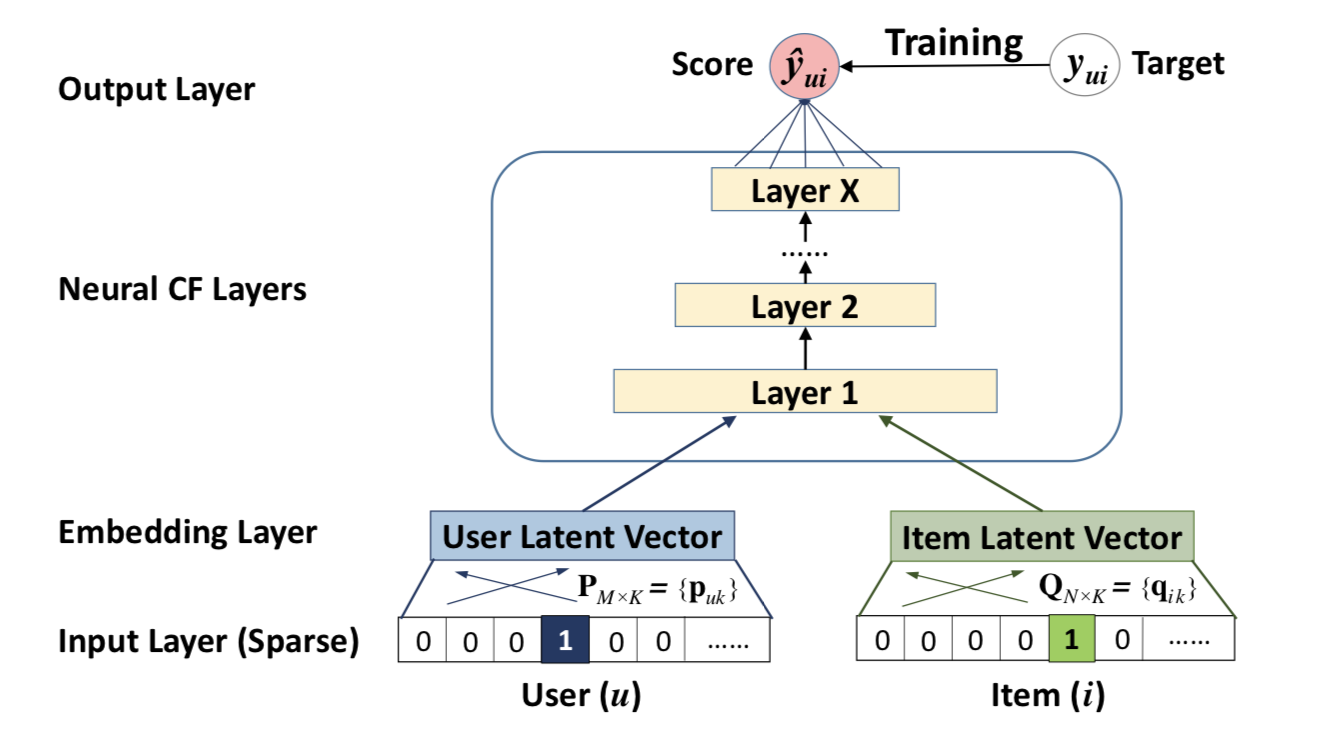
\includegraphics[width=0.9\columnwidth]{NCF.png}
	\caption{Neural collaborative filtering framework.}
	\label{fig:ncf}
	\vspace{-10pt}
\end{figure}
It uses a log-likelihood funciton as the loss function to train the model,
\begin{equation}
    \begin{aligned} L &=-\sum_{(u, i) \in \mathcal{Y}} \log \hat{y}_{u i}-\sum_{(u, j) \in \mathcal{Y}^{-}} \log \left(1-\hat{y}_{u j}\right) \\ &=-\sum_{(u, i) \in \mathcal{Y} \cup \mathcal{Y}^{-}} y_{u i} \log \hat{y}_{u i}+\left(1-y_{u i}\right) \log \left(1-\hat{y}_{u i}\right) \end{aligned}
\end{equation}
whose optimization is done by performing stochastic gradient descent (SGD).

The second one is DELF \cite{cheng2018delf}, a dual-embedding based deep latent factor 
model for recommendation. This model take a dual view from both user-side and
item-side. It not only uses the user's interacted items, but also item's interacted
users. By utilizing dual side information to better model the relationship
between the target user and the target item. Furthermore, DELF employs an 
attention mechanism to discriminate the importance of interacted 
users/items for dual-embedding learning. Another novel attempt of the model 
is modeling the user-item interactions with four deep representations, and a fusion
layer is used to subtly fuse the information of the four representations.
The framework of DELF is shown in Fig. ~\ref{fig:delf}.
\begin{figure}[h]
	\centering
	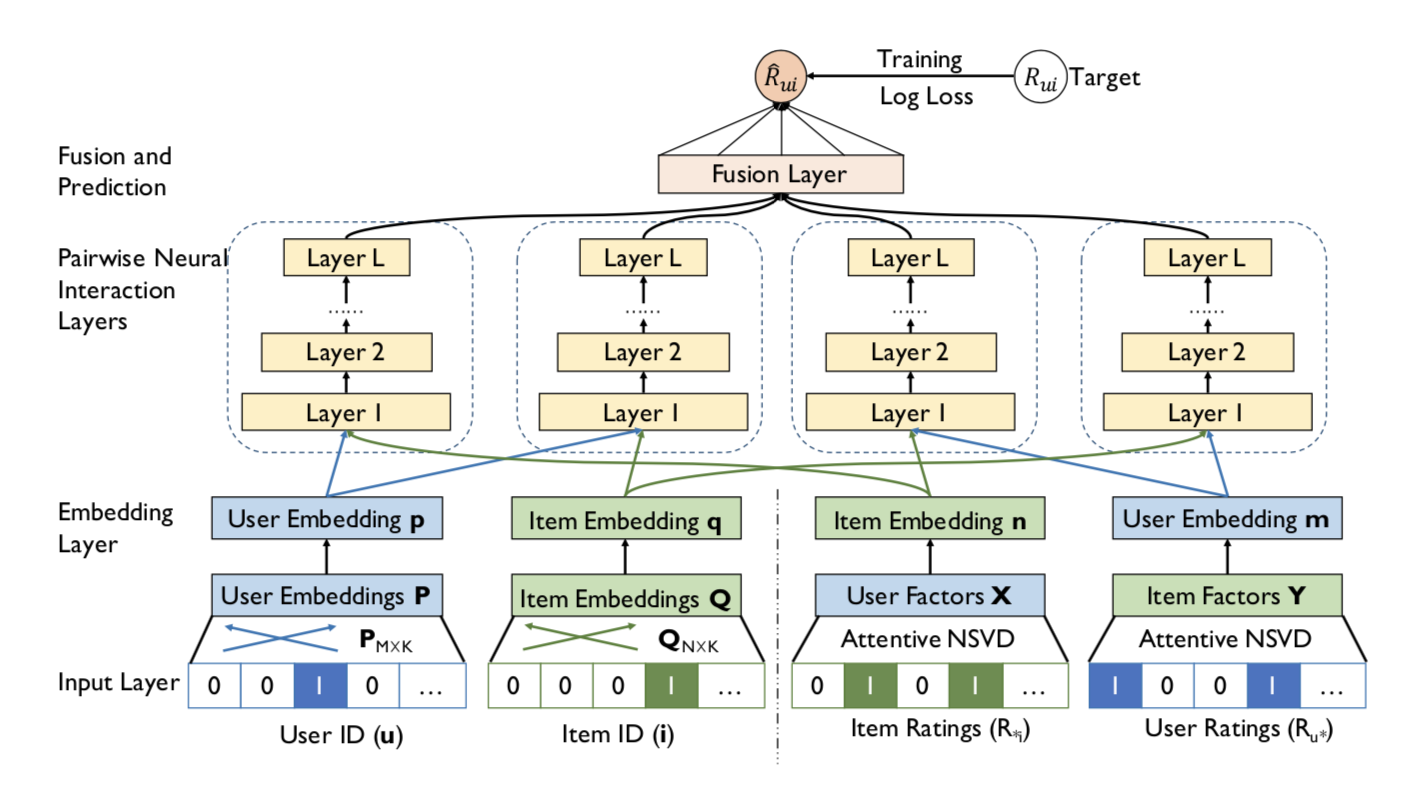
\includegraphics[width=0.9\columnwidth]{DELF.png}
	\caption{DELF framework.}
	\label{fig:delf}
	\vspace{-10pt}
\end{figure}

In this model, the item-based user dense representation $m_u$ is modeled as,
\begin{equation}
    \mathbf{m}_{u}=\sum_{i \in R(u)} \alpha_{i} \mathbf{y}_{i}
\end{equation}
where $\alpha_{i}$ is the attention value which indicates the importance of
the interacted item. The attention value is calculated as,
\begin{equation}
    \begin{aligned} \mathbf{h}_{i} &=\tanh \left(\mathbf{W}_{a} \mathbf{y}_{i}+\mathbf{b}_{a}\right) \\ \alpha_{i} &=\frac{\exp \left(\mathbf{h}_{i}^{T} \mathbf{h}_{a}\right)}{\sum_{i \in R(u)} \exp \left(\mathbf{h}_{i}^{T} \mathbf{h}_{a}\right)} \end{aligned}
\end{equation}
where $W_a$, $b_a$ denote the weight matrix and bias vector respectively, and
$h_a$ is the context vector.
Similarly, it represent the target item with user factors as,
\begin{equation}
    \mathbf{n}_{i}=\sum_{u \in R(i)} \alpha_{u} \mathbf{x}_{u}
\end{equation}
where the users that have interacted with the target item are aggregated as
a user-based item representation. This is the "dual" view of DELF which is 
attentional.

To model the complex feature interactions between $u$ and $i$, DELF uses a 
pairwise neural interaction layer instead of using a single network structure.
It models the user-item interactions in a seperate way, formally,
\begin{equation}
\begin{array}{c}{\mathbf{h}^{j}=\phi_{L}^{j}\left(\ldots \phi_{2}^{j}\left(\phi_{1}^{j}\left(\mathbf{z}_{0}[j]\right)\right) \ldots\right)} \\ {\phi_{l}^{j}=\delta_{l}^{j}\left(\mathbf{W}_{l}^{j} \mathbf{z}_{l-1}^{j}+\mathbf{b}_{l}^{j}\right), l \in[1, L]} \\ {\mathbf{z}_{0}=\left[\mathbf{p}_{u} \oplus \mathbf{n}_{i}, \mathbf{p}_{u} \oplus \mathbf{q}_{i}, \mathbf{m}_{u} \oplus \mathbf{n}_{i}, \mathbf{m}_{u} \oplus \mathbf{q}_{i}\right]}\end{array}
\end{equation}
where $j \in \{1,2,3,4\}$; $h_j$ is the deep representation of embedding representation
which is learned by $j$-th pairwise interaction neural network.
The fusion and prediction layer is defined as,
\begin{equation}
\begin{array}{c}{\mathbf{h}_{f}=\delta_{f}\left(\mathbf{W}_{f} \mathbf{z}_{f}+\mathbf{b}_{f}\right)} \\ {\mathbf{z}_{f}=\mathbf{h}^{1} \oplus \mathbf{h}^{2} \oplus \mathbf{h}^{3} \oplus \mathbf{h}^{4}}\end{array}
\end{equation}
and the prediction function is
\begin{equation}
    \hat{R}_{u i}=\delta_{p}\left(\mathbf{W}_{p} \mathbf{h}_{f}+b_{f}\right)
\end{equation}


\section{Sequential User Modeling}
One key aspect of recommender system is user modeling, i.e. to capture the latent interests of the user and derive the adaptive representation for each user\cite{zhou2018deepa,zheng2017joint}.
Recently, sequential user modeling has drawn huge attention since the sequences of user behaviors have rich information for the user interests, especially for concept drifting \cite{widmer1996learning}, long-term behavior dependency \cite{koren2009collaborative,ren2019lifelong}, periodic patterns \cite{ren2018repeatnet}, etc.

There are three categories for sequential user modeling.
The first one is from the view of temporal collaborative filtering \cite{koren2009collaborative} with the consideration of drifting user preferences.
The second stream is based on Markov-chain methodology \cite{rendle2010factorizing,he2016fusing,he2016vista} which implicitly models the user state dynamics and derive the outcome behaviors.
The third school is based on deep neural networks, such as recurrent neural networks (RNN) \cite{hidasi2015session,hidasi2017recurrent,wu2017recurrent,jing2017neural,liu2016context,beutel2018latent,villatel2018recurrent} and convolutional neural networks (CNN) regarding the behavior history as an image \cite{tang2018personalized,kang2018self}.
However, most of these methods only care about user's interest drifting and do not consider the sequential patterns of items, which also deliver rich information for user-item matching.
Furthermore, most of these sequential models only care about user's own interaction history while ignore the information that could be found in similar users or items.

In the following subsections, we describe the methods of third school using deep neural
networks in details.
\subsection{RNN-based Models}
\subsection{CNN-based Models}
\subsection{Attention-based Models}

\section{Graph Pattern Mining in Recommender Systems}
In the domain of recommender systems, there are two schools of graph pattern mining methods.

The first school of models make use of additional information such as social networks \cite{song2019session,wu2019dual} or knowledge graphs \cite{wang2018ripplenet} to enhance the learning process of user-user relations or item-item relations respectively. These models are tricky since they use other side information which may not be easy to obtain.

The second school only uses user-item bipartite interaction graph.
The perspective of bipartite graph is novel for recommender system \cite{fadel2018link}, which could be facilitated by the recent advances of graph pattern mining \cite{kipf2016semi} and link prediction in graph domain \cite{van2017graph}.
\cite{niu2018collaborative} utilize the graph information of both the target user and the target item for better collaborative filtering while they ignore the temporal dynamics of the evolving graphs.
\cite{wu2017recurrent} use RNNs to do sequence modeling for both user and item side. However, the model applies simple sum-pooling on the interacted items/users in each time slice thus not effective.
The model proposed in \cite{fadel2018link} captures spatial graph patterns along timeline with graph convolutional networks (GCN) \cite{van2017graph}. However, they just consider the first-order relations without collaborative information among the graphs.

In the following subsections, we describe the methods of the two schools in details.

\subsection{Social Network-based Models}
\subsection{Knowledge Graph-based Models}
\subsection{User-item Bipartite Graph-based Models}
\chapter{Methodology}\label{sec:method}
In this section, we first define the problem and present some preliminaries. Then we discuss our proposed model in detail and the connection between our model and the other existing works.

\begin{table}[t]
	% \renewcommand{\arraystretch}{1}
	\centering
	\caption{Notations and descriptions}\label{tab:notation}
	\resizebox{\columnwidth}{!}{
		\begin{tabular}{c|l}
			\hline
			Notation & Description. \\
			\hline
			$u, v$ & The target user and the target item. \\
			$M, N$ & The number of users and items. \\
			$y, \hat{y}$ & The indicator and the predicted probability of the user-item interaction. \\
			$\bm{u}, \bm{v}$ & Dense representation of target user $u$ and target item $v$.\\
			$\mg_t^k(u), \mg_t^k(v)$ & K-hop \textit{user/item-rooted interaction set} at time slice $t$.\\
			$\mg_t(u), \mg_t(v)$ & \textit{user/item-rooted interaction set} at time slice $t$.\\
			$\mg^t(\cdot)$ & The incremental graph at the $t$-th time slice.\\
			% $\bm{E}_{\mg_t^k(u)}, \bm{E}_{\mg_t^k(v)}$ & Dense representations of items/users in $\mg_t^k(u)$ and $\mg_t^k(v)$.\\
			% $e$ & Dense representation of user (or item) in $\mg_t^k(u)$ (or $\mg_t^k(v)$).\\
			$\bm{u}_t^{k}, \bm{v}_t^{k}$ & Aggregated user/item-side representation of k hop(s) graph information \\
			& at time slice $t$.\\
			$U, V$ & User/item-side sequence.\\
			$\Delta T$ & Time interval to split subgraphs.\\
			$S$ & Size of \textit{user/item-rooted interaction set}.\\
			\hline
		\end{tabular}
	}
\end{table}

\begin{figure*}[t]
	\centering
	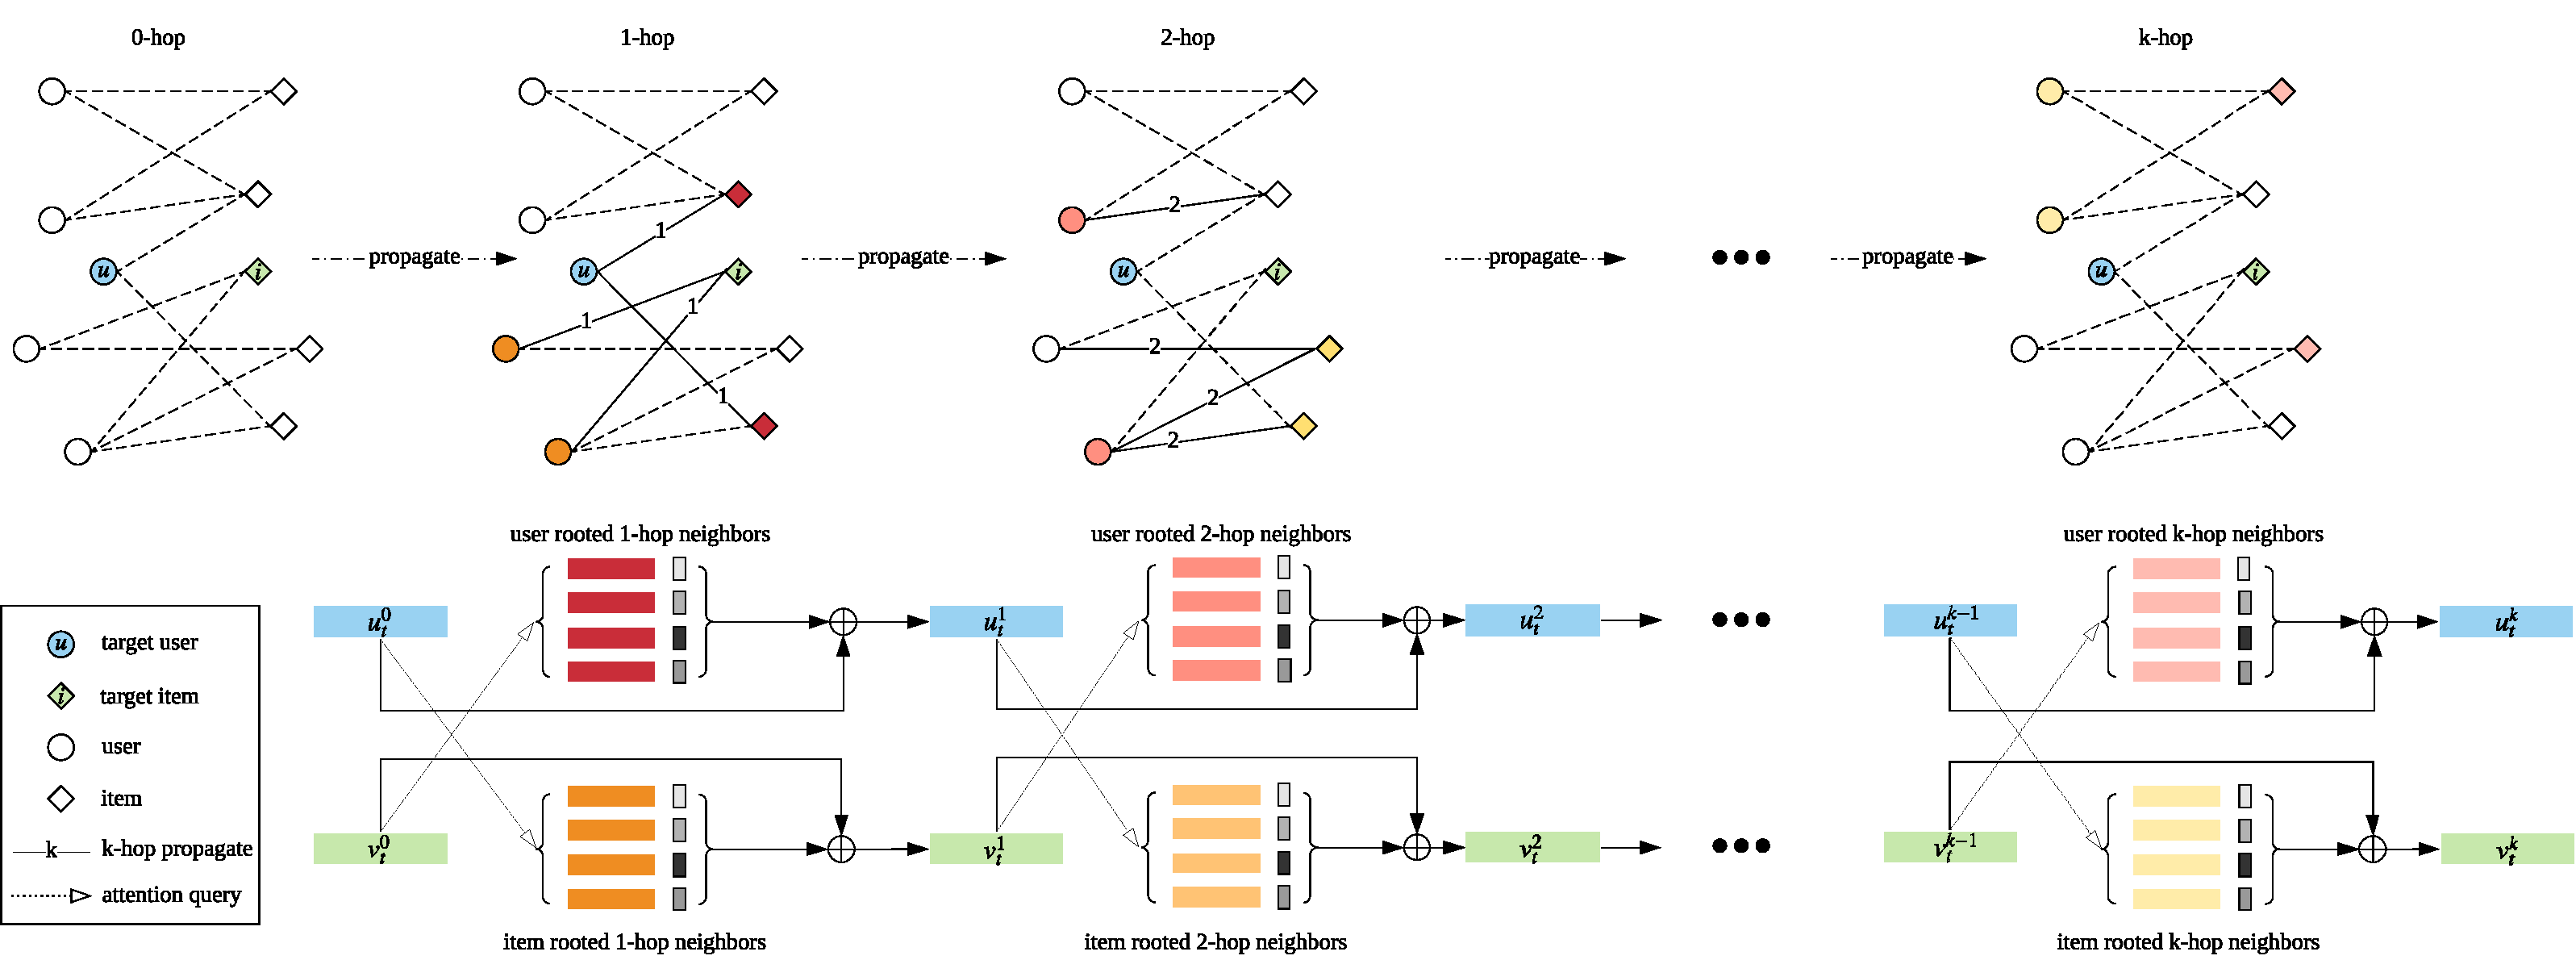
\includegraphics[width=1.0\textwidth]{score_spatial.pdf}
	\caption{Multi-hop Co-Attention Graph Network calculation process.}
	\label{fig:spatial-framework}
	\vspace{-10pt}
\end{figure*}

\section{Preliminaries}\label{sec:preliminaries}
In a recommender system, there are $M$ users in $\mathcal{U}=\{u_1, \ldots, u_M\}$ and $N$ items in $\mathcal{V}=\{v_1, \ldots, v_N\}$.
We regard the user-item interactions as a bipartite graph $\mg$ whose nodes are users and items while its edges are interactions defined as
% In the history, any user may reveal interests on some items and the interaction behaviors would be tracked in the system as $\mathcal{Y}=\{y_{uv} | u \in \mathcal{U}, v \in \mathcal{V} \}$ and
\begin{equation}
	y_{ij} = \left\{
		\begin{array}{rcl}
			1, & & i~(\text{user}/\text{item})~ \text{has interacted with} ~j~(\text{item}/\text{user}); \\
			0, & & \text{otherwise.} \\
		\end{array}
	\right.
\end{equation}
The user-item interaction $y$ is either implicit feedback \cite{agarwal2009spatio}, i.e., clicks or explicit user rating \cite{koren2009collaborative}.
Without loss of generality, we focus on the implicit feedback which is more common in practice\cite{zhou2018deepa,ren2019lifelong,guo2017deepfm}.

\subsection{User/Item-Rooted Interaction Set}
From a start node on the graph, we could take multiple hops, and gather a series of nodes which are the neighbors of the start node with different distance. 

Hereby we define \textit{user-rooted interaction set} of the target user $u$ at distance $k$ hops as
\begin{equation}
\mg^k(u) = \{j|y_{ij}=1, i \in \mg^{k-1}(u) \}
\end{equation}
and $\mg^{0}(u) = \{u\}$ which contains only the root node. Symmetrically, we define \textit{item-rooted interaction set} of the target item $v$ as 
\begin{equation}
\mg^k(v) = \{j|y_{ij}=1, i \in \mg^{k-1}(v) \}
\end{equation}
and $\mg^{0}(v) = \{v\}$.

There is some collaborative information retrieved through this propagation process. As for the view of user, the k-hop \textit{user-rooted interaction set} $\mg^k(u)$ contains item nodes ($k=2n-1, n \in N^{+}$) and user nodes when $k = 2n, n \in N^{+}$. The items in $\mg^k(u)$ and $\mg^{k+2}(u)$ both attract the same group of users that are in $\mg^{k+1}(u)$, while the users in $\mg^{k+1}(u)$ and $\mg^{k+3}(u)$ demonstrate similar interests on the items in $\mg^{k+2}(u)$. 
These collaborative patterns are useful for the subsequent modeling.
%These relations that users share same intersts and items show similar attractions are the \textbf{collaborative} information that we may use for the subsequent modeling.
And the situation of the target item is symmetrically similar. 

We combine all the information obtained through $K$-hop propagation to form the \textit{user-rooted interaction set} and \textit{item-rooted interaction set} as $\mg(u) = \bigcup_{k=0}^K \mg^k(u)$ and $\mg(v)=\bigcup_{k=0}^K \mg^k(v)$.
% \subsection{Interaction Set}
% % graph
% Given the target user $u$, we can conduct the \textit{interaction set} of user $u$ as
% \begin{equation}
% \mg(u) = \{v_i | y_{uv_i}=1 \}.
% \end{equation}
% The user's interaction set is the collection of all the items that the user has interacted with.
% From the view of the user-rooted interaction graph, we may regard $\mg_u$ as the 1-hop neighboring nodes from the root node $u$, as is illustrated in Figure~\ref{fig:bi-graph}.

% It is natural to expand the user-rooted interaction graph and find the \textit{co-interaction set} as
% \begin{equation}
% 	\mg(v|u) = \{ u_j | y_{{u_j}{v_i}}=1, v_i \in \mg_u \}.
% \end{equation}
% The co-interaction set includes all the users who have also interacted with the items in $\mg(u)$, i.e., they may share the similar tastes with the user $u$.
% From the view of graph, all the users in $\mg(v|u)$ are represented as the nodes through 2-hop from the root user $u$.
% Here we only care about the interaction and co-interaction sets of $u$ and we have omitted the other interaction connections through multi-hop ($>2$) relations from the root user, since it may bring more noise than useful patterns. In many works of GNN, using 2-hop neighbors is good enough.\jiarui{citation of GNN work}

% The above disscussion is from the user side, while we may also define the interaction set $\mg(v)$ and the co-interaction set $\mg(u|v)$ of the given item $v$ from the item side with similar definition.
% The differences lie in the meaning of the ``interaction'' where, from the item side, the items in the co-interaction set $\mg(u|v)$ share the similar properties to the given item $v$ for they have interactions with same group of users.

\subsection{Evolving Interaction Graph}
Now that we have defined the local interaction graph $\mg$ of the user $u$ and the item $v$, we take one step forward and consider the incremental evolving interaction graphs along the time to capture temporal dynamics of both user and item.
%For example, during a specific time period, the users may make several interactions with some items; 
Specifically, the users (items) may conduct different interactions with other items (users) at different time.
Thus, the whole interaction graph is evolving all the time and consisted of several incremental subgraphs.

To better model the dynamic temporal patterns of the interaction graphs, we slice the whole graph to $T$ sliced subgraphs, each of which is constructed within a unified time interval. So that
\begin{equation}
\begin{aligned}
	\mg(\cdot) &= \bigcup_{t=1}^T \mg_t(\cdot), \\
\end{aligned}
\end{equation}
where $\mg_t(\cdot)$ contains all the interactions happened during the $t$-th time slice.
Specifically, the \textit{user-rooted interaction set} at $t$-th time slice is denoted as $\mg_t(u)$ and the \textit {item-rooted interaction set} is $\mg_t(v)$

\subsection{Task Definition}
The goal of the recommender system is to estimate the probability of interactions $\hat{y}$ between the target user $u \in \mathcal{U}$ and the given item $v \in \mathcal{V}$, with consideration of the user-rooted subgraph $\mg_u$ and the item-rooted subgraph $\mg_v$ as
\begin{equation}
\hat{y}_{uv} = \mathit{f}(u, v| \mg_u, \mg_v; \btheta)
\end{equation}
through the learned function $\mathit{f}$ with parameters $\btheta$ where $\mg_u = \bigcup_{t=1}^T \mg_t(u)$ and $\mg_v=\bigcup_{t=1}^T \mg_t(v)$.
We conclude the notations and the corresponding description in Table~\ref{tab:notation}.



\section{Spatial Graph Pattern Mining}\label{sec:spatial}
In this section, we describe the proposed \textit{Co-Attention Graph Network} for handling the user/item-rooted subgraphs. We also present an importance sampling strategy used to retrieve more related neighbors while avoiding noise.


\subsection{Co-Attention Graph Network}
At each time slice $t$, we use \textit{Co-Attention Graph Network} to aggregate subgraph information. We take the view of the target user $u$ as an example.
The propagated information of different user (or item) nodes in $\mg^k_t(u)$ would contribute differently to the final recommendation decisions.
Traditional method like GAT \cite{velivckovic2017graph} and \cite{song2019session} utilize the spatial information of the local graph through calculating attentional relatedness between the center node and its nearest neighboring nodes, which has no relevance to the target item and may be unsuitable for recommender system.
%Take $\mg^1_t(u)$ as an example, the items in $\mg^1_t(u)$ should be weighted by the target item $v$ instead of their center node $u$. And it is not suitable when we consider the multi-hop senario. \jiarui{how to express that this bottom-up way is not suitable for recommendation domain?}

To address this problem, we propose \textit{Co-Attention Graph Network}. As illustrated in~Fig \ref{fig:spatial-framework}, for the k-th hop propagation, we calculate user-side representation and item-side representation as
\begin{equation}
\bm{u}_t^k = \bm{u}_t^{k-1} + \sum_i \alpha_{ui}^k e_i^k ~,
\end{equation}
\begin{equation}
\bm{v}_t^k = \bm{v}_t^{k-1} + \sum_i \alpha_{vi}^k e_i^k ~,
\end{equation}
where $e_i^k$ is the $d$-dimensional dense embedding of users (or items) in the k-hop \textit{user/item-rooted interaction set}. And We set $\bm{u}_t^0 = \bm{u}$, $\bm{v}_t^0 = \bm{v}$. The co-attention weights $\alpha_{ui}^k$ and $\alpha_{vi}^k$ are calculated as

\begin{equation} \label{eq:co_atten_1}
\alpha_{ui} = \frac{exp(LeakyReLU(\bm{a^T}[\bm{We}_i^k||\bm{Wv_t^{k-1}}]))}{\sum_{\bm{e}_j^k \in \mg^k(u)}exp(LeakyReLU(\bm{a^T}[\bm{We}_j^k||\bm{Wv_t^{k-1}}]))}
\end{equation}

\begin{equation}  \label{eq:co_atten_2}
\alpha_{vi} = \frac{exp(LeakyReLU(\bm{a^T}[\bm{We}_i^k||\bm{Wu_t^{k-1}}]))}{\sum_{\bm{e}_j^k \in \mg^k(v)}exp(LeakyReLU(\bm{a^T}[\bm{We}_j^k||\bm{Wu_t^{k-1}}]))}
\end{equation}
Here $\bm{W} \in R^{d \times d}$ is weight matrix of a shared linear transformation which applied to every node's representation. $||$ is a concatenate operation, $\bm{a} \in R^{2d \times 1}$ is the weight vector of a single-layer feedforward neural network with LeakyReLU activation function which is
\begin{equation}
%y_{ij} = \left\{
%\begin{array}{rcl}
%1, & & i~(\text{user}/\text{item})~ \text{has interacted with} ~j~(\text{item}/\text{user}); \\
%0, & & \text{otherwise.} \\
%\end{array}
%\right.
	LeakyReLU(x) = \left\{
		\begin{array}{ccr}
		x, x \geq 0; \\
		\frac{x}{\gamma}, x < 0,
		\end{array}
	\right.
\end{equation}
where negative input slop $\gamma = 0.2$. Then it is normalized by softmax function.

Please note that we use an iterative way to aggregate multi-hop information. The target item's representation $\bm{v}_t^{k-1}$ from the last iteration, i.e., $(k - 1)$-hop, is used as a query to calculate the co-attention weight values of the $k$-th hop neighbors of the target user $u$. 
$\bm{v}_t^{k-1}$ contains not only the target item's own information, but the collaborative information of its neighbors from all the previous $(k - 1)$ hops.
And we make symmetrically the similar operation for the target item.
%the target item's side uses user representation as attention query. 
In this way, the representations of both the target user and the target item are correlated and collaborative. This collaborative view from both sides to do graph learning is proved an effective way in the experiments in Section~\ref{sec:ab-study}.

% \subsubsection{Co-Attention Mechanism for 2-hop Neighbors}
% In this section, we describe the co-attention mechanism that is used to utilize 2-hop spatial information. We need to find collaborative relations between two groups of nodes: one group is the users in $\mg(v)$ and $\mg(v|u)$, the other is the items in $\mg(u)$ and $\mg(u|v)$, as is illustrated in Figure~\ref{fig:framework}.

% Take $\mg(u)$ and $\mg(v|u)$ as an example, $\bm{E}_{\mg(u)} \in R^{K_1 \times d}$ and $\bm{E}_{\mg(v|u)} \in R^{K_2 \times d}$ are embedding matrix of $\mg(u)$ and $\mg(v|u)$ respectively. The affinity matrix $\bm{C} \in R^{K_1 \times K_2}$ is calculated as 
% \begin{equation}
% 	\bm{C} = F_p(\bm{E}_{\mg(u)}) \bm{A} (F_q(\bm{E}_{\mg(v|u)}))^T
% \end{equation}
% where $F_p(\cdot)$ and $F_q(\cdot)$ are one-layer neural network functions with ReLU activation function for $\bm{E}_{\mg(u)}$ and $\bm{E}_{\mg(v|u)}$ respectively and $\bm{A} \in R^{d \times d}$ is an attentive matrix.

% After calculating the affinity matrix $\bm{C}$, we conduct max-pooling (MP) operation along rows of $\bm{C}$ respectively to generate importance vector $\bm{a}^{col} \in R^{K_2 \times 1}$ for $\bm{E}_{\mg(v|u)}$, and the importance vector is then normalized by softmax function.
% \begin{equation}
% 	\bm{a}_j^{col'} = MP(\{\bm{C}_{ij}\}_{i=1}^{K_1})%\bm{a}_i^{row'} = MP(\{\bm{C}_{ij}\}_{j=1}^{K_2}),~~~
% \end{equation}
% \begin{equation}
% 	\bm{a}^{col} = Softmax(\bm{a}^{col'})%\bm{a}^{row} = Softmax(\bm{a}^{row'}),~~~
% \end{equation}
% So, the aggregated representation of user-side 2-hop neighbors is
% \begin{equation}
% 	\bm{u}^{(2)}_t = \sum_{j \in [0, K_2-1]} \bm{a}_j^{col} * \bm{E}_{\mg(v|u)}^j
% \end{equation}
% where $\bm{E}_{\mg(v|u)}^j$ is the j-th row of the embedding matrix.

% In a symmetric way, we can get the item-side 2-hop neighbors representation $\bm{v}^{(2)}_t$.
% % explain the meaning of the co-attention calculation
% By using the co-attention mechanism, we give the relevant 2-hop neighbors more attention than those that are not very relevant so that the noise introduced by the 2-hop expansion can be reduced.
% In this way, we effectively utilize the 2-hop spatial information and find relations between user rooted subgraph and item rooted subgraph at each time slice.

\subsection{Importance Sampling Strategy with Local Graph Structure}\label{sec:sampling}
When we do the $k$-th propagation from $\mg_t^{k-1}(u)$ (or $\mg_t^{k-1}(v)$), there could be a lot of nodes in $\mg_t^k(u)$ and it could introduce too much noise. Thus we need an importance sampling strategy for each propagation process.
% which will sample the most relative nodes in the next hop.
When doing sampling, we could regard the \textit{user/item-rooted subgraph} as a directed graph, the direction is the propagation direction from $(k-1)$-th hop to $k$-th hop, as the propagation from $\mg^{k-1}_t(u)$ to $\mg^k_t(u)$ which is illustrated in Fig.~\ref{fig:sampling}.

We calculate the importance factor of node $p$ in $\mg^k_t(u)$ as
\begin{equation}
	\bm{I}_p = \sum_{q \in pre(p)} \frac{1}{\textit{out-degree}(q)}
\end{equation}
where $pre(p)$ contains the predecessor nodes of node $p$ (which is $\mg^{k-1}_t(u)$ in Fig.~\ref{fig:sampling}).
Then the importance factors are normalized by a softmax function and used as sampling probabilities as 
\begin{equation}
	\bm{Pr}_p = \frac{\exp(\bm{I}_p)}{\sum_{n\in \mg^{k}_t(u)} \exp(\bm{I_n})} ~.
\end{equation}

If a node in $\mg^k_t(u)$ has more predecessors, it indicates that the node is more important and more related to the previous nodes. However, if the predecessor is very popular (out-degree is large), then the relatedness from this predecessor is reduced. 
The reason to punish the predecessor nodes with their popularity is the following: when we consider the nodes in $\mg^{k-2}_t(u)$ which are the same type to the nodes in $\mg^k_t(u)$ (both are users or items), relation though a very popular intermedia node (in $\mg^{k-1}_t
(u)$) is not that important than a relation though a not popular intermedia node. In this way, we could find more similar and related collaborative nodes in $\mg^{k}_t(u)$.
%\kan{needs refine.}


\begin{figure}[h]
	\centering
	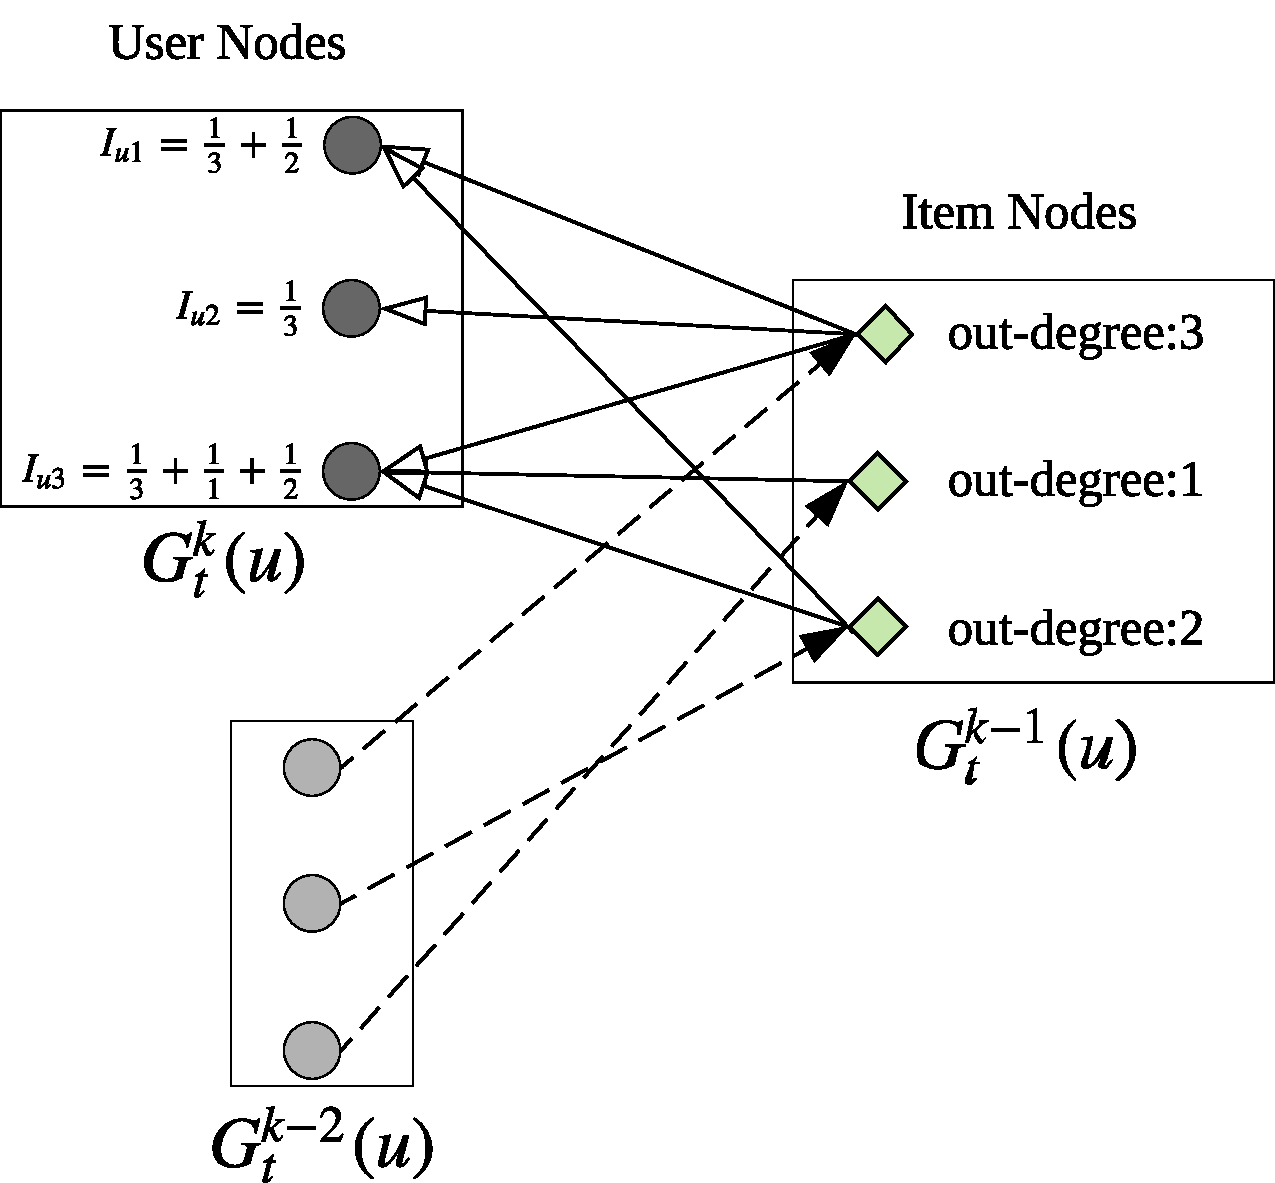
\includegraphics[width=0.7\columnwidth]{importance_sampling.pdf}
	\caption{Illustration of importance sampling of $\mg_t^k(u)$.}
	\label{fig:sampling}
	\vspace{-10pt}
\end{figure}
% \subsubsection{Co-Attention Mechanism}\label{sec:co-atten}
% We first formulate and present co-attention mechanism that we use in our model\cite{hu2018local}. $\bm{P} \in R^{m \times d}$ and $\bm{Q} \in R^{n \times d}$ are the two sets which need to be jointly represented. The affinity matrix $\bm{C} \in R^{m \times n}$ is calculated as
% \begin{equation}
% 	\bm{C} = F_p(\bm{P}) \bm{A} (F_q(\bm{Q}))^T
% \end{equation}
% where $F_p(\cdot)$ and $F_q(\cdot)$ are multi-layer neural network functions for $\bm{P}$ and $\bm{Q}$ respectively and $\bm{A} \in R^{d \times d}$ is an attentive matrix.

% After calculating the affinity matrix $\bm{C}$, we conduct max-pooling (MP) operation along rows and columns of $\bm{C}$ respectively to generate importance vectors for $\bm{P}$ and $\bm{Q}$.
% \begin{equation}
% 	\bm{a}_i^p = MP(\{\bm{C}_{ij}\}_{j=1}^n),~~~\bm{a}_j^q = MP(\{\bm{C}_{ij}\}_{i=1}^m)
% \end{equation}
% Then we conduct softmax function on both $\bm{a}^p$ and $\bm{a}^q$ and get normalized importance vectors.
% Finally, we use the normalized importance vectors to perform weighted sum on $\bm{P}$ and $\bm{Q}$ and get final representations as
% \begin{equation}
% 	\bm{p} = \bm{P}^T \bm{a}^p, ~~~\bm{q} = \bm{Q}^T \bm{a}^q
% \end{equation}
% \subsubsection{Use of Co-Attention}
% Co-attention mechanism is used to mining spatial relations and aggregate the graph information within one time slice. We use embedding mechanism to map each item and user to a low-dimensional space, so user-side 1-hop sub graph $\mg^t(u)$ and item-side 2-hops sub graph $\mg^t(v|u)$ are mapped to relative embedding matrices. And the embedding matrices are used as the $\bm{P}$ and $\bm{Q}$ in \ref{sec:co-atten} relatively and the two sub graphs are represented as $\bm{u}_t^{(1)}$ and $\bm{v}_t^{(2)}$. Similarly, $\mg^t(v)$ and $\mg^t(u|v)$ are treated in the same way, so we get $\bm{v}_t^{(1)}$ and $\bm{u}_t^{(2)}$ relatively.


\section{Temporal Interactive Dual Sequence Modeling} \label{sec:temporal}
As the sequential recommendation task can be regarded as a dynamic graph link prediction problem described in Section~\ref{sec:preliminaries}, in this section, we describe the method we use to model the temporal incremental graphs and the proposed \textit{Interactive Attention} used for dual sequence modeling.

\subsection{Temporal Dynamics of Incremental Graphs}
For each time slice, we get the representations of target user $u$ and target item $v$ as $\bm u_t^K$ and $\bm v_t^K$, respectively. These representations are the results after $K$ hops propagation and aggregation which is described in Section~\ref{sec:spatial}.
After that we get two sequences $U$ and $V$, which are the sequences of target user's and item's multi-hop representation respectively. For simplicity, we denote $\bm u_t = \bm u_t^K$ and $\bm v_t = \bm v_t^K$ and
\begin{equation}
U = \{\bm{u}_1, \bm{u}_2, ..., \bm{u}_{T}\}~,
V = \{\bm{v}_1, \bm{v}_2, ..., \bm{v}_{T}\} .
\end{equation}

We use Gated Recurrent Unit \cite{cho2014learning} (GRU) to model the temporal dynamics for  target user-side and target item-side. Each GRU model takes the corresponding graph representation $\bm u_t^K$ at each time step and the hidden state $\bh_{t-1}$ from the last time step, and then calculates as
\begin{equation}\small
\begin{aligned}
\bm{z}_t^u =& ~\sigma (\overline{\bm{W}}_z^u \bm{u}_t + \overline{\bm{U}}_z \bh_{t-1}^u + \overline{\bm{b}}_z^u) \\
\bm{r}_t^u =& ~\sigma (\overline{\bm{W}}_r^u \bm{u}_t + \overline{\bm{U}}_r \bh_{t-1}^u + \overline{\bm{b}}_r^u) \\
\bh_{t}^u =& ~(1 - \bm{z}_t^u) \odot \bh_{t-1}^u  \\
&~~~~~~~~~~~~~~~~~+ \bm{z}_t^u \odot \tanh(\overline{\bm{W}}_h^u \bm{u}_t + \overline{\bm{U}}_h^u (\bm{r}_t^u \odot \bh_{t-1}^u) + \overline{\bm{b}}_h^u)  ~,
\end{aligned}
\label{eq:gru}
\end{equation}
where $\odot$ is the element-wise product operator. 

The item-side temporal dynamics are modeled in the same way. Till now, we've got user-side and item-side sequence of temporal nodes representations: $\{\bm h_1^u, \bm h_2^u, ..., \bm h_T^u\}$ and $\{\bm h_1^v, \bm h_2^v, ..., \bm h_T^v\}$.

\subsection{Interactive Attention Mechanism of Dual Sequence} \label{sec:attention}
As illustrated in Fig~\ref{fig:temporal-framework}, different time slice has different impact on the final prediction at $T + 1$. And hereby we introduce our \textit{Interactive Attention Mechanism}. Unlike the attention mechanism in \cite{zhou2018deepb} and \cite{zhou2018deepa} which uses target item to query the interacted items sequence, we utilize dual sequences information at the same time interactively to weigh across different time slice.
The attention value of each time slice $\beta_t$ is calculated as,
\begin{equation}
relation_t = \sigma(\bm Q_2(\sigma(\bm Q_1((\bm h_t^u \odot \bm h_t^v) || (\bm u \odot \bm v)))))
\end{equation}

\begin{equation}
\beta_t = \frac{\exp(relation_t)}{\sum_{i=1}^T \exp(relation_i)}
\end{equation}
where $\sigma$ is ReLU activation function and $\bm Q_1$, $\bm Q_2$ are weight matrix of the two-layer MLP.

And the final representations of target user and target item are 
\begin{equation} \label{eq:seq_rep}
\bm r_u = \sum_{t=1}^T \beta_t \bm h_t^u, ~~~~\bm r_v = \sum_{t=1}^T \beta_t \bm h_t^v
\end{equation}

In this way, we utilize dual sequences information to calculate attention weights which reflect interaction intensity of each time slice. Different from common attention mechanism used in sequential recommendation/user response prediction task \cite{zhou2018deepb, zhou2018deepa} which uses target item as query and retrieve the most relevant user historical behaviors, we model the relations between target user and item at each time slice interactively from both sequences and give them different importance. The effectiveness of the proposed \textit{Interactive Attention} is shown in Section.~\ref{sec:ab-study}.

\begin{figure}[t]
	\centering
	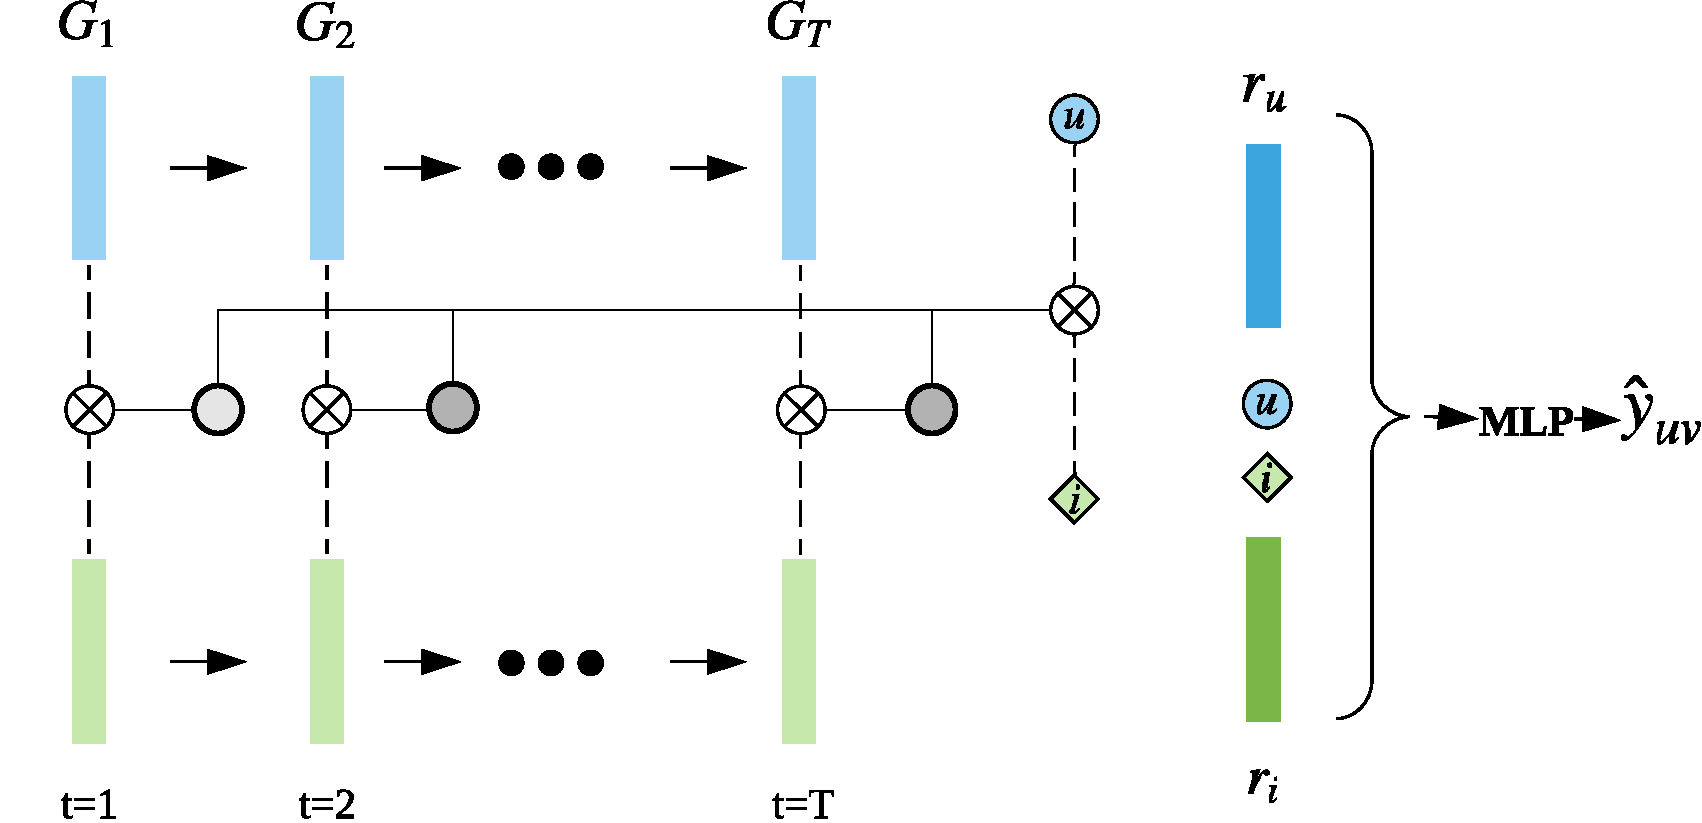
\includegraphics[width=1.0\columnwidth]{score_temporal.pdf}
	\caption{Temporal Interactive Dual Sequence Modeling of SCoRe.}
	\label{fig:temporal-framework}
	\vspace{-10pt}
\end{figure}


\section{Final Prediction and Loss Functions}
The predicted probability of interaction between the target user and the target item is calculated as
\begin{equation}
\hat{y} = f(\bm{r}_u, \bm{r}_v, \bm{u}, \bm{v}; \bm{\Theta}),
\end{equation}
where $f$ is implemented as a multi-layer perceptron with the ReLU activation function. The parameters set of the MLP is $\bm{\Theta}$.
The inference procedure is illustrated in Figure~\ref{fig:temporal-framework}.

As for the loss function, we take an end-to-end training and introduce (i) the widely used cross entropy loss $\mathcal{L}_{\text{ce}}$ \cite{ren2018bid,zhou2018deepa,zhou2018deepb} over the whole training dataset with (ii) the parameter regularization $\mathcal{L}_{\text{r}}$. We utilize stochastic gradient descent for optimization. Thus the final loss function is
\begin{equation}
\begin{aligned}
\argmin_{\bm{\Theta}, \bm{\Phi}} &= \mathcal{L}_{\text{ce}} + \lambda \mathcal{L}_r \\
&= -\sum_{s} \big[ y_s \log \hat{y}_s + (1-y_s) \log (1-\hat{y}_s)\big] \\
& + \frac{1}{2} \lambda \left( \|\bm{\Theta} \|_2^2 + \| \bm{\Phi} \|_2^2 \right) ~,
\end{aligned}
\end{equation}
where $\bm{\Phi}$ includes the parameters in GRUs, $\bm{W}$, $\bm{a}$ in \textit{Co-Attention Graph Network} and $\bm Q_1$, $\bm Q_2$ of \textit{Interactive Attention Mechanism}.

\section{Relations to Previous Works}
The proposed model can be simplified to previous frameworks of recommender systems:

\begin{itemize}[leftmargin=15pt]
	\item \textbf{Dual Sequence Framework:} If we only use 1-hop neighbors of the target user and the target item, as $u_t = u_t^1$ and $v_t = v_t^1$, and treat each neighbor and each time slice equally, \score~ would have the same structure as RRN \cite{wu2017recurrent} and GCMC \cite{fadel2018link}.
	\item \textbf{Single Sequence Framework:} If we eliminate the item-side sequence from the dual sequence framework above and make each time slice only has one interaction, we might get the framework of sequential recommendation models similar to RNN models \cite{hidasi2015session,ren2019lifelong,zhou2018deepb}.
	\item \textbf{Non Sequence Framework:} If we don't consider the temporal dynamics of user interests of the above single sequence framework, and consider the user behaviors as a whole, then \score~ might degenerate to the traditional CF models \cite{koren2008factorization}.
\end{itemize}
\chapter{Experiments}\label{sec:exps}{}
In this section, we present the details of the experiment setups and the corresponding results. To illustrate the effectiveness of our proposed model, we compare it with some strong baselines on sequential recommendation task. Moreover, we have published our reproductive code\footnote{https://bit.ly/2WZWTKC}.

We start with three research questions (RQ) to lead the experiments and the following discussions.
\begin{itemize}
	\item [\textbf{RQ1}] Compared to the baseline models, does SCoRe achieve state-of-the-art performance in sequential recommendation task?
	\item [\textbf{RQ2}] What is the influence of different components in~\score? Is the sampling method described in Section~\ref{sec:sampling} useful?
	\item [\textbf{RQ3}] What patterns does the proposed model capture for the final recommendation decision?
\end{itemize}

\section{Experimental Setups}
In this part, we describe our experiment setups including datasets with preprocessing method, some important implementation details, evaluation metrics and the compared baselines.
\subsection{Datasets}
We use three real-world large-scale datasets to evaluate all the compared models. The dataset statistics have been shown in Table ~\ref{tab:dataset-statistics}.
\begin{description}[leftmargin=15pt]
	\item [CCMR] \cite{cao2016complete} is a dataset consists of movie rating logs collected from Douban, which is one of China's largest movie review websites. The data is collected and dumped in May 2015.
	\item [Tmall] \footnote{https://tianchi.aliyun.com/dataset/dataDetail?dataId=42} is provided by Alibaba Group which contains user behavior history on Tmall e-commerce platform from May 2015 to November 2015.
	\item [Taobao] \cite{zhu2018learning} is a dataset consisting of user behavior data collected from Taobao\footnote{https://tianchi.aliyun.com/dataset/dataDetail?dataId=649}, one e-commerce platform in China. It contains user behaviors from November 25 to December 3, 2017 of several behavior types including click, purchase, add to cart and item favoring.
\end{description}

\noindent\textbf{Dataset Preprocessing}.
As we consider the user-item interactions as a sequence of bipartite graphs, we cut it into total $T$ time slices with the same time interval as shown in Table~\ref{tab:dataset-statistics}. And for each time slice, we use the interaction records within it to construct the user-item bipartite graph.
In every sliced graph, we start from the target user/item node and step out for $K$ hops to get the \textit{user/item-rooted interaction set} and the interaction sets of every time slice form the user/item-side sequences. 
We set $K=2$ for the three datasets.

\begin{table}[t]
	%	\scriptsize
	\centering
	\caption{The dataset statistics.}\label{tab:dataset-statistics}
	%	\vspace{-10pt}
	\resizebox{\columnwidth}{!}{
		\begin{tabular}{c|r|r|r|r|r}
			\hline
			Dataset & Users \# & Items \# & Interaction \# & Time slices \# & Time interval $\Delta T$\\
			\hline
			CCMR & 4,920,695 & 190,129 & 283,775,314 & 41 & 90 days\\
			\hline
			Tmall & 424,170 & 1,090,390 & 54,925,331 & 13 & 15 days\\
			\hline
			Taobao & 987,994 & 4,162,024 & 100,150,807
			 & 9 & 1 day\\
			\hline
		\end{tabular}
	}
%	\vspace{-10pt}
\end{table}

% \jiarui{add figures about how many 1-hop/2-hop neighbor a user/item has at each time slice, ccmr vs taobao/tmall item side differences}

\noindent\textbf{Positive \& Negative Samples}.
To evaluate the recommendation performance, we use one positive item and sample 100 negative items at the prediction time $T + 1$ for each user in all three datasets.
For Tmall and Taobao datasets, as we only have the positive user feedbacks (click, buying, etc.), we have to randomly sample the negative items. As for CCMR datasets, we regard items whose ratings are 5 or 4 as positive items and those whose ratings are 1,2 or 3 as negative items. If a user does not have enough negative items, we use random sampling to generate negative items for her.

\noindent\textbf{Train \& Test Splitting}.
The training set contains the sequential behaviors from 1st to $(T-1)$th time slice, we use the interactions history from 1 to $T-2$ to predict the interactions in $(T-1)$. For the testing set, we use the interactions data from 1 to $T-1$ to predict the interactions in $T$.

\noindent\textbf{Implementation Details}.
It is common that the target user doesn't have any interaction record in a time slice, and similarly, the target item may be not visited by any user in a time slice. To handle this issue, we use a unified embedding vector to represent these users and items.

We set the size of all the k-hop \textit{user/item-rooted interaction sets} to $S$ which can be regarded as a hyperparameter.
For each hop's neighbors, we follow the sampling strategy described in Section~\ref{sec:sampling}.% and the sampling happens for every data sample when it is fed to the model which means it could be different nodes in \textit{user/item-rooted interaction set} for the same data sample during training.


\subsection{Evaluation Metrics}
Three evaluation metrics are used and all of them are widely used in recommendation tasks.

\textbf{HR@k} (\textit{Hit Ratio@k}) measures the proportion of samples that the positive item is among the top-k in all test cases which is computed as,
\begin{equation}
HR@k = \frac{1}{|\mathcal{U}|} \sum_{u \in \mathcal{U}} \mathbb I (R_{u, v} \leq k),
\end{equation}
where $R_{u,v}$ is the ranking position of the user $u$'s interacting with item $v$, and $\mathbb I$ is the indicator function.

\textbf{NDCG@k} (Normalized Discounted Cumulative Gain) is a position-aware metric which assigns larger weights on higher ranks of the positive item, which is calculated as,
\begin{equation}
NDCG@k = \frac{1}{|\mathcal{U}|} \sum_{u \in \mathcal{U}} \frac{2^{\mathbb I (R_{u, v} \leq k)} - 1} {log(R_{u, v} + 1)}.
\end{equation}

\textbf{MRR} (Mean Reciprocal Rank) is another position-aware metric that is calculated as,
\begin{equation}
MRR = \frac{1}{|\mathcal{U}|} \sum_{u \in \mathcal{U}} \frac{1}{R_{u, v}}.
\end{equation}

% Because we just have one positive item per user, HR@k is equal to Recall@k and it is linear to Precision@k, while MRR is equal to Mean Average Precision (MAP). 
As HR@1 is equal to NDCG@1, so in this work, we report HR@\{1,5,10\}, NDCG@\{5,10\} and MRR in detail.

 
\subsection{Compared Baselines}\label{sec:comp-models}
To illustrate the effectiveness of our model, we compare \score ~with two CF models, three sequential recommendation models and two graph-based models.
We follow \cite{zhou2018deepb} that all the models take the input sparse features and feed them through an embedding layer for the subsequent inference.

The first group of models are CF models:
\begin{itemize}[leftmargin=40pt]
	\item [\textbf{SVD++}] \cite{koren2008factorization} is a hybrid method of latent factor model and neighbor-based model which is the fundamental approach of collaborative filtering recommendation. It regards all the sequential behaviors as a whole and ignores the temporal dynamics.
	\item [\textbf{DELF}] \cite{cheng2018delf} is the state-of-the-art CF method which utilizes deep neural networks to capture complex non-linear interaction patterns from both user-side and item-side.
\end{itemize}

The second group is sequential recommendation methods, which are based on RNNs, CNNs, or Transformer architecture:
\begin{itemize}[leftmargin=40pt]
	\item [\textbf{GRU4Rec}] \cite{hidasi2015session} bases on GRU and it is the first work using the recurrent cell to model sequential user behaviors.
	\item [\textbf{Caser}] \cite{tang2018personalized} is based on CNNs that uses horizontal and vertical convolutional filters to capture user behavior patterns at different scales.
	\item [\textbf{SASRec}] \cite{kang2018self} bases on Transformer \cite{vaswani2017attention}, it only uses self-attention mechanism without recurrent architecture. It achieves very competitive performance in sequential recommendation task.
\end{itemize}

The third group is graph-based sequential recommendation models. For fair comparison, we use the same time interval to do time slicing.
\begin{itemize}[leftmargin=40pt]
	\item [\textbf{RRN}] \cite{wu2017recurrent} is the first RNN-based model that considers both the user- and item-side sequence. It uses sum-pooling to aggregate the information inside a time slice which can be regarded as a graph-based model.
	\item [\textbf{GCMC}] \cite{fadel2018link} is a link prediction model based on sequential bipartite graph for recommender system. It uses graph structured data for final prediction. GCMC is a method for matrix completion using Graph Convolutional Networks (GCNs) to handle dynamic graphs. 
	\item [\textbf{SCoRe}] is our proposed model which is described in Section~\ref{sec:method}.
\end{itemize}

\begin{table}[t]
	%	\scriptsize
	\centering
	\caption{The hyperparameter settings of \score. $h$ is hidden vector size. $\eta$ is learning rate, $b$ is batch size.}\label{tab:hyperparas}
	%	\vspace{-10pt}
	\resizebox{0.9\columnwidth}{!}{
		\begin{tabular}{c|l}
			\hline
			CCMR & $d=16$, $h=32$, $K=2$, $S=5$, $\eta=0.0005$, $b=100$, $\lambda=0.005$\\
			Tmall & $d=16$, $h=32$, $K=2$, $S=10$, $\eta=0.001$, $b=200$, $\lambda=0.0005$\\
			Taobao & $d=16$, $h=32$, $K=2$, $S=10$, $\eta=0.001$, $b=200$, $\lambda=0.0001$\\
			\hline
		\end{tabular}
	}
	\vspace{-10pt}
\end{table}

\subsection{Hyperparameter Settings}
The hyperparameters are determined by optimizing MRR on test set. The detailed hyperparameters of \score~ are listed in Table~\ref{tab:hyperparas}. For fair consideration, the latent dimension of all compared baselines remain the same, while the other hyperparameters of all the baselines are set based on grid search in the same search space.


\begin{table*}[h]
	\centering
	\caption{Performance comparison against baseline models. Bold values are the best in each row, while the second best values are underlined. Improvements over baselines are statistically significant with $p$ < 0.01. HR, NDCG, MRR: the higher, the better)}\label{tab:perf-table}
	\tiny
	\resizebox{0.9\textwidth}{!}{
		\begin{tabular}{c|c|cc|ccc|ccc}%ccc|ccc}
			\hline
			\multirow{2}{*}{Dataset} & \multirow{2}{*}{Metric} & \multicolumn{2}{c|}{Group 1} & \multicolumn{3}{c|}{Group 2} & \multicolumn{3}{c}{Group 3}\\
			& & SVD++ & DELF & GRU4Rec & Caser & SASRec & RRN & GCMC & \score\\
			\hline
			\multirow{6}{*}{CCMR} & HR@1 & 0.2378 & 0.6536 & 0.6703 & 0.6777 & \underline{0.6979} & 0.6633 & 0.6591 & \textbf{0.7001}\\
			& HR@5 & 0.4288 & 0.9087 & 0.8911 & 0.8907 & 0.9047 & 0.903 & \underline{0.9063} & \textbf{0.9118} \\
			& HR@10 & 0.5462 & 0.9586 & 0.9268 & 0.9184 & 0.9361 & 0.9469 & \underline{0.9508} & \textbf{0.9583} \\
			& NDCG@5 & 0.3356 & 0.7919 & 0.7917 & 0.7954 & \underline{0.8123} & 0.7957 & 0.7946 & \textbf{0.8161} \\
			& NDCG@10 & 0.3735 & 0.8084 & 0.8034 & 0.8045 & \underline{0.8226} & 0.8101 & 0.8092 & \textbf{0.8281} \\
			& MRR & 0.3375 & 0.7617 & 0.7662 & 0.7699 & \underline{0.7878} & 0.7681 & 0.7652 & \textbf{0.7913} \\
			\hline
			\hline
			\multirow{6}{*}{Tmall} & HR@1 & 0.1229 & 0.2001 & 0.1979 & 0.2029 & 0.3312 & 0.4177 & \underline{0.4254} & \textbf{0.4764} \\
			& HR@5 & 0.3098 & 0.3765 & 0.3818 & 0.4037 & 0.6307 & \underline{0.6452} & 0.6449 & \textbf{0.6806} \\
			& HR@10 & 0.3438 & 0.4573 & 0.4713 & 0.4925 & 0.7072 & 0.7449 & \underline{0.7512} & \textbf{0.7632} \\
			& NDCG@5 & 0.2112 & 0.2975 & 0.2947 & 0.3089 & 0.4935 & 0.5368 & \underline{0.5403} & \textbf{0.5842} \\
			& NDCG@10 & 0.2342 & 0.3130 & 0.3236 & 0.3376 & 0.5184 & 0.5691 & \underline{0.5747} & \textbf{0.6109} \\
			& MRR & 0.1373 & 0.2990 & 0.2950 & 0.3058 & 0.4676 & 0.5257 & \underline{0.5314} & \textbf{0.5734} \\
			\hline
			\hline
			\multirow{6}{*}{Taobao} & HR@1 & 0.0705 & 0.1299 & 0.1117 & 0.1292 & 0.1897 & 0.2138 & \underline{0.2164} & \textbf{0.2431} \\
			& HR@5 & 0.1539 & 0.2999 & 0.3001 & 0.3022 & 0.3871 & \underline{0.4695} & 0.4672 & \textbf{0.4991} \\
			& HR@10 & 0.2063 & 0.4656 & 0.4395 & 0.4539 & 0.5331 & \underline{0.6213} & 0.6156 & \textbf{0.6467} \\
			& NDCG@5 & 0.0998 & 0.1719 & 0.1667 & 0.1724 & 0.2512 & 0.3447 & \underline{0.3449} & \textbf{0.3590} \\
			& NDCG@10 & 0.1082 & 0.2008 & 0.1995 & 0.2013 & 0.2788 & \underline{0.3937} & 0.3929 & \textbf{0.4112} \\
			& MRR & 0.0935 & 0.1203 & 0.1119 & 0.1232 & 0.2198 & 0.3402 & \underline{0.3411} & \textbf{0.3786} \\
			\hline
		\end{tabular}
	}
	% \vspace{-10pt}
\end{table*}

\section{Evaluation Results: RQ1} \label{sec:comp_results}
% \kan{the influence of sparsity in data is an issue. we should discuss about it.}

The experimental results are shown in Table~\ref{tab:perf-table}, we find several observations that:
\begin{itemize}[leftmargin=15pt]
	\item By comparing the performance of \score~ and other baseline models, it outperforms baselines by 134.5\% to 0.4\%, 317.6\% to 7.9\% and 304.9\% to 11.0\% on MRR in CCMR, Tmall and Taobao dataset, respectively. And it also shows significant improvements on the other metrics so \score~ achieves the state-of-the-art performance in sequential recommendation task.
	\item For the models in Group 1, they do not consider the temporal dynamics of user behaviors thus perform not so good as models in Group 2 and 3. DELF uses both user-side and item-side interaction information so it achieves better performance than SVD++ which only utilizes user-side information.
	\item By comparing the performance of Group 2 and 3, we find in Tmall and Taobao dataset that, Group 3 outperforms Group 2 over CCMR dataset, SASRec and Caser are better than Group 3. As shown in Table~\ref{tab:dataset-statistics}, Tmall and Taobao has a lot more items than CCMR, which makes ranking items more difficult in Tmall and Taobao. So it is more important on these two datasets to take item-side sequence into consideration because it gives the models more information than just using single user-side sequence. 
	\item SASRec achieves satisfactory performance, especially compared to the other models in Group 1/2. It is accounted for utilizing the effective self-attention mechanism and more supervision signals at each time point.
	\item GCMC performs better than RRN in many cases. It may because that RRN just simply apply sum-pooling over the neighbors' information at each time slice, while GCMC uses graph convolution network to better capture the neighbors' information.
\end{itemize}

\textbf{Influence from the size of \textit{user/item-rooted interaction set}}.
We vary the size of \textit{user/item-rooted interaction set} of each hop to further investigate the robustness of \score. The results are shown in Table~\ref{tab:size-perf-table}. 
We find that when size increases, the performance is improved at first because that the larger the size is, the more information it contains. And when the size continues to increase, the performances begin to drop which indicates that too much noise and useless information is introduced.

\begin{table}[h]
	\centering
	\caption{Performance comparison on different size of \textit{user/item-rooted interaction set.}}\label{tab:size-perf-table}
	\tiny
	\resizebox{0.9\columnwidth}{!}{
		\begin{tabular}{c|c|cccc}
			\hline
			\multirow{2}{*}{ Dataset } & \multirow{2}{*}{ Metric } & \multicolumn{4}{c}{ Size of Interaction Set } \\
			& & 5 & 10 & 15 & 20 \\
			\hline
			\multirow{3}{*}{ CCMR } & HR@10 & \textbf{0.9583} & 0.9555 & 0.9498 & 0.9423 \\
			& NDCG@10 & \textbf{0.8281} & 0.8239 & 0.8232 & 0.8221 \\
			& MRR & \textbf{0.7913} & 0.7909 & 0.7895 & 0.7829 \\
			\hline
			\multirow{3}{*}{ Tmall } & HR@10 & 0.7589 & \textbf{0.7632} & 0.7619 & 0.7607 \\
			& NDCG@10 & 0.6091 & \textbf{0.6109} & 0.6087 & 0.6052 \\
			& MRR & 0.5658 & \textbf{0.5734} & 0.5698 & 0.5611 \\
			\hline
			\multirow{3}{*}{ Taobao } & HR@10 & 0.6288 & \textbf{0.6467} & 0.6319 & 0.6299 \\
			& NDCG@10 & 0.4068 & \textbf{0.4112} & 0.4081 & 0.4027 \\
			& MRR & 0.3679 & \textbf{0.3786} & 0.3673 & 0.3648 \\
			\hline
		\end{tabular}
	}
	\vspace{-10pt}
\end{table}


\section{Ablation Study: RQ2} \label{sec:ab-study}
In this section, we conduct some ablation studies to investigate the effectiveness of four important components of \score~: (1) \textit{Interactive Attention Mechanism} in dual sequences modeling; (2) \textit{Co-Attention Graph Network} for spatial information aggregation; (3) The consideration of using multi-hop instead of just one hop. (4) The importance sampling strategy which is used to find more relevant neighbors and reduce noise.

%\begin{figure}[h]
%	\centering
%	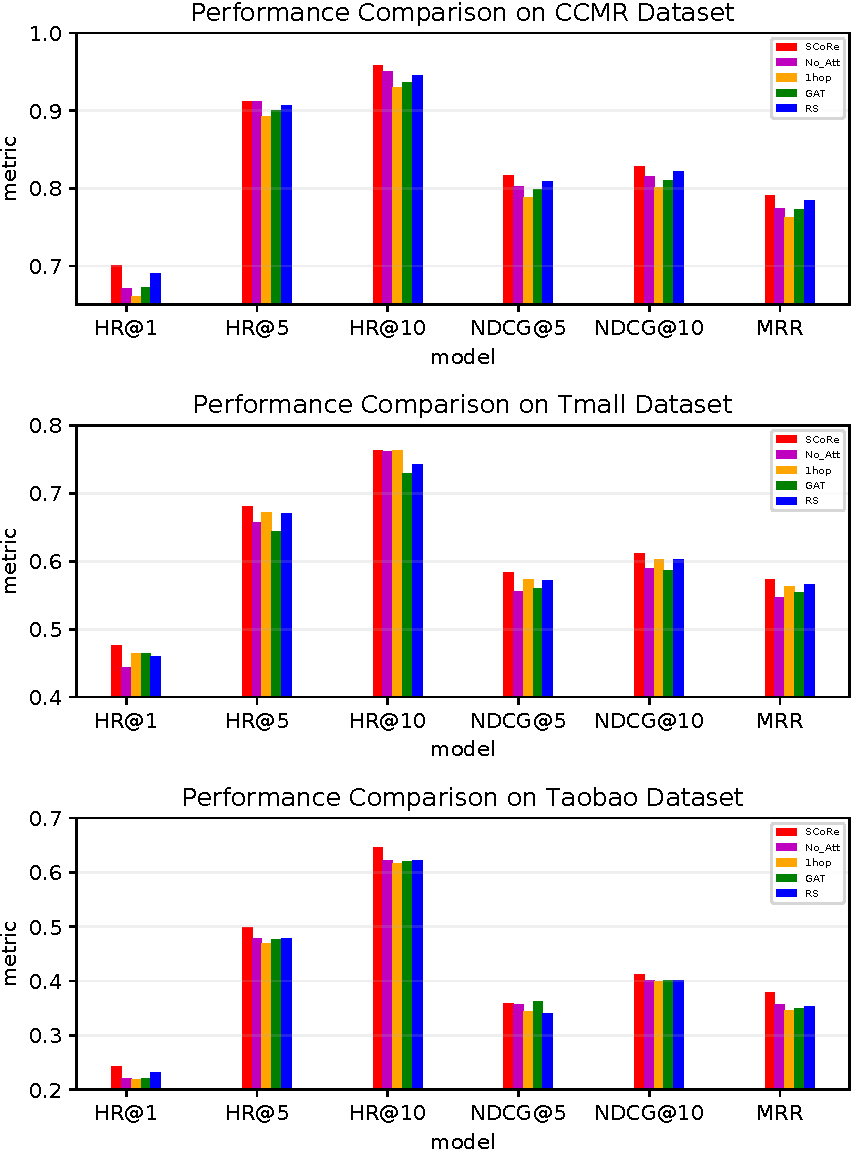
\includegraphics[width=0.9\columnwidth]{figures/ab_study.pdf}
%	\caption{Performance Comparison of Ablation Study.}
%	\label{fig:ab_study}
%	\vspace{-10pt}
%\end{figure}

\begin{table}[h]
	\centering
	\caption{Performance comparison of ablation study} \label{tab:ab_study_table}
	\tiny
	\resizebox{\columnwidth}{!}{
		\begin{tabular}{c|c|ccccc}
			\hline
			\multirow{2}{*}{ Dataset } & \multirow{2}{*}{ Metric } & \multicolumn{5}{c}{ models }\\
			& & RIA & Single-hop & GAT & RS & \score \\
			\hline
			\multirow{3}{*}{ CCMR } & HR@10 & 0.9509 & 0.9296 & 0.9358 & 0.9452 & \textbf{0.9583} \\
			& NDCG@10 & 0.8157 & 0.8011 & 0.8104 & 0.8217 & \textbf{0.8281} \\
			& MRR & 0.7741 & 0.7621 & 0.7724 & 0.7841 & \textbf{0.7913} \\
			\hline
			\multirow{3}{*}{ Tmall } & HR@10 & 0.7620 & 0.7632 & 0.7287 & 0.7431 & \textbf{0.7632} \\
			& NDCG@10 & 0.5893 & 0.6029 & 0.5866 & 0.6032 & \textbf{0.6109} \\
			& MRR & 0.5567 & 0.5633 & 0.5543 & 0.5662 & \textbf{0.5734} \\
			\hline
			\multirow{3}{*}{ Taobao } & HR@10 & 0.6216 & 0.6172 & 0.6201 & 0.6212 & \textbf{0.6467} \\
			& NDCG@10 & 0.4001 & 0.3991 & 0.4017 & 0.4015 & \textbf{0.4112} \\
			& MRR & 0.3575 & 0.3456 & 0.3498 & 0.3523 & \textbf{0.3786} \\
			\hline
		\end{tabular}
	}
%	\vspace{-10pt}
\end{table}


\begin{figure*}[h]
	\centering
	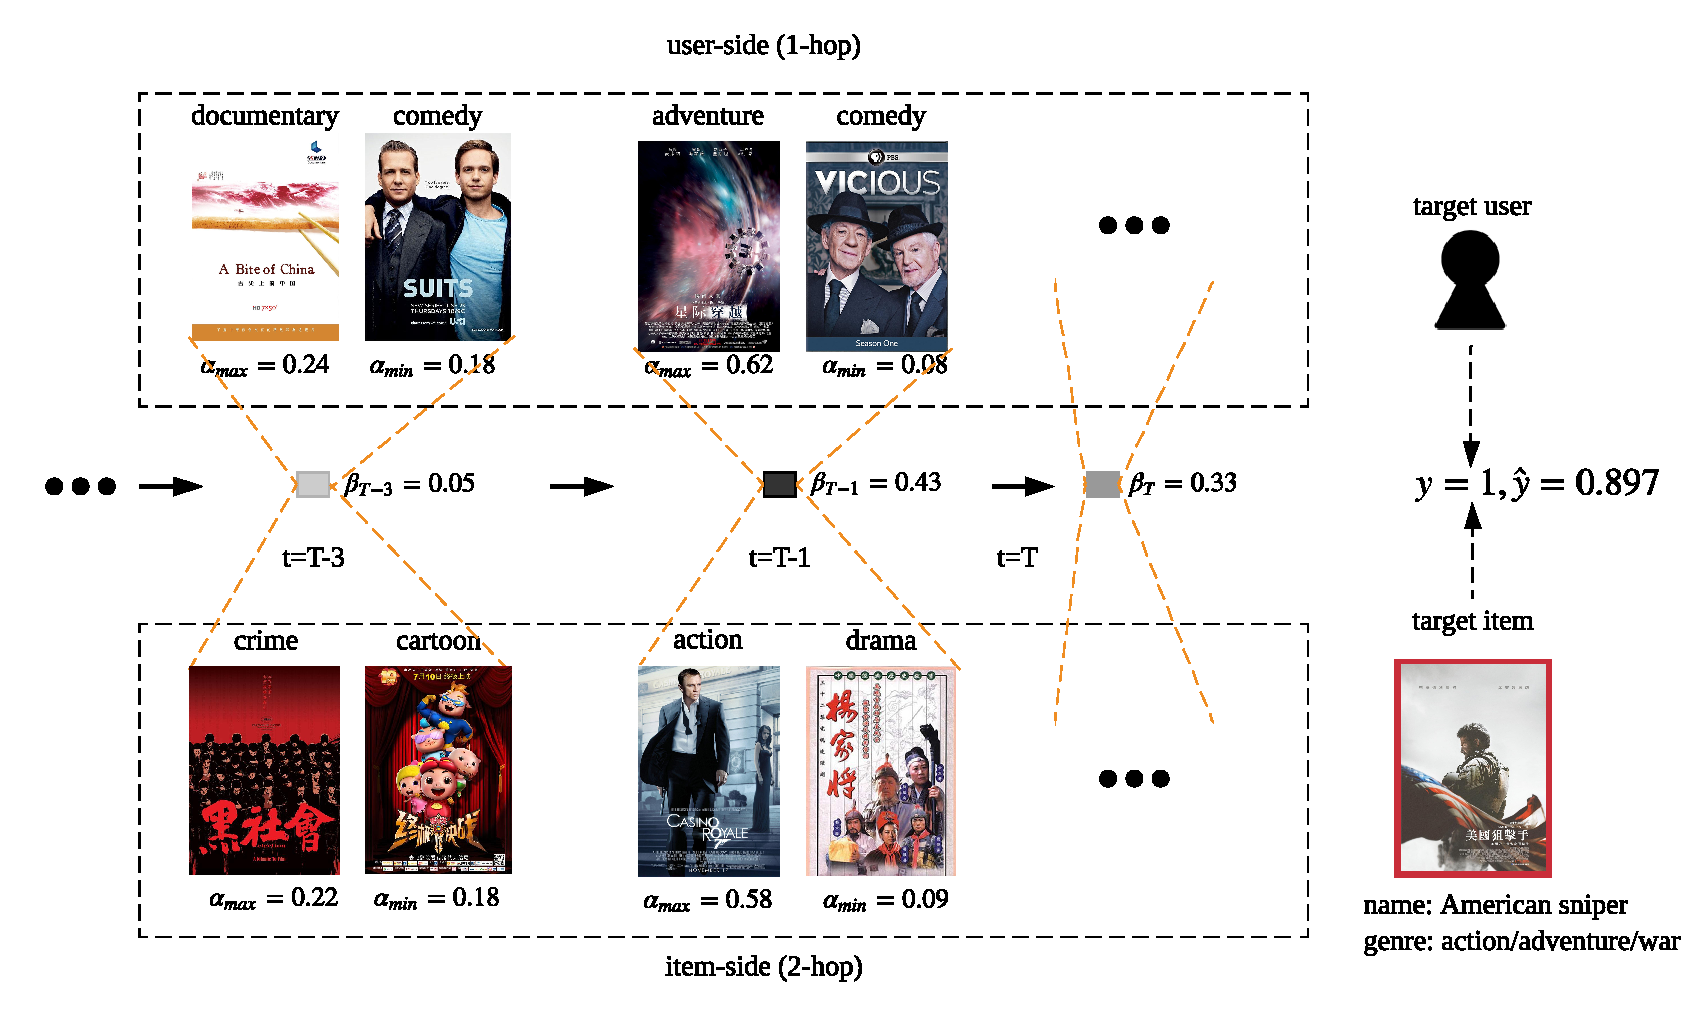
\includegraphics[width=0.8\textwidth]{visual.pdf}
	\caption{Visualization analysis of patterns that are captured by \score.}
	\label{fig:visual}
	\vspace{-10pt}
\end{figure*}

We set four comparative settings, and the performances of them have been shown in Table~\ref{tab:ab_study_table}.
The details of the four settings are listed as below.
\begin{itemize}[leftmargin=15pt]
	\item \textbf{RIA} (Remove Interactive Attention) removes the attention part described in~\ref{sec:attention} and set the final sequential representations of target user and item as $\bm r_u = h_T^u$ and $\bm r_v = h_T^v$ of Eq.~(\ref{eq:seq_rep}).
	\item \textbf{Single-hop} only uses the 1-hop neighbors of the target user and item that $\mg_t(u) = \mg^1_t(u)$ and $\mg_t(v) = \mg^1_t(v)$.
	\item \textbf{GAT} uses Graph Attention Network proposed in \cite{velivckovic2017graph}. We use this model to evaluate the effectiveness of the proposed \textit{Co-Attention Graph Network}.
	\item \textbf{RS} (Random Sampling) is the same as \score, but it uses random sampling instead of importance sampling described in Section~\ref{sec:sampling}.
\end{itemize}
Except for the changes mentioned above, the other parts of the models and experiment settings remain identical to that above to ensure fair comparison.

Except for the changes mentioned above, the other parts of the models and experimental settings remain identical to ensure the fairness of comparison.

From Table~\ref{tab:ab_study_table} we can find that (1) in CCMR and Taobao dataset, Single-hop performs worse than RIA and GAT but performs better than them in Tmall datasets. It indicates that the \textit{Interactive Attention} and \textit{Co-Attention Graph Network} are critical architectures to aggregate multi-hop neighbors. Simply adding multi-hop neighbors without the two mechanisms above may not have a better performance. (2) RIA performs better than GAT over most of the metrics on all the datasets. It shows that our proposed graph information aggregator is more effective than GAT in the recommendation domain. (3) RS outperforms the other ablation models which means \score~ is robust regardless of how the neighbor nodes are sampled. (4) \score~performs the best against all the four ablation models which shows the effectiveness of our proposed method for both spatial (\score~vs GAT) and temporal (\score~vs RIA) modeling, and the experimental results prove that importance sampling is helpful to the model performance.

\section{Visualization: RQ3}
In this section, we further investigate what patterns \score~captures by studying and visualizing a specific case sampled from the CCMR dataset. 

As is shown in Fig.~\ref{fig:visual}, the target item is a movie named "American Sniper" whose genre is ``action, adventure and war''. The value of \textit{Interactive Attention} $\beta_{T-1}$ and $\beta_{T-3}$ are plotted and $\beta_{T-1} = 0.43$ is the maximum value while $\beta_{T-3} = 0.05$ is a smaller value which indicates that the graph information in $(T-1)$ is the most important to the final prediction ($y=1$, and prediction value $\hat{y}=0.897$ ). However, the information retrieved during the $(T-3)$-th time slice has less contribution to the prediction.

We look deeper at what happened during the $(T-3)$th and the $(T-1)$th time slice.
We plot the items (aka, movies) in 1-hop \textit{user-rooted interaction set} and 2-hop \textit{item-rooted interaction set} in Fig.~\ref{fig:visual}. 
Recall that the 1-hop \textit{user-rooted interaction set} contains the target user's direct interests, and the 2-hop \textit{item-rooted interaction set} contains the items that attract the same group of users as the target item at the same time slice. We plot the maximum and minimum of co-attention values calculated in Eq.~\ref{eq:co_atten_1} and Eq.~\ref{eq:co_atten_2} with the corresponding item information. The item with maximum co-attention value is the most relevant one in the interaction set while the minimum co-attention value corresponds to the least relevant item.
From Fig.~\ref{fig:visual} we find that: 
\begin{itemize}[leftmargin=15pt]
	\item In the $(T-3)$th time slice, neither 1-hop \textit{user-rooted interaction set} nor 2-hop \textit{item-rooted interaction set} contains relative items to the target item, they contains comedy, cartoon or crime movies. So the attention values are almost the same across all items in an interaction set, and there is little useful information at $(T-3)$ as indicated by the small value of $\beta_{T-3}$.
	\item In the $(T-1)$th time slice, on the contrary, 1-hop \textit{user-rooted interaction set} contains a relative item ("Interstellar" which is an adventure and fiction movie) and it is given maximum co-attention value, which is calculated with the target item representation $\bm{v}_{T-1}^0(=\bm{v})$. Furthermore, the 2-hop \textit{item-rooted interaction set} contains a even more relative item ("007" which is an action and adventure movie) and it has max attention value. This attention value is calculated with $u^1_{T-1}$ which encodes the information of the 1-hop \textit{user-rooted interaction set} described above (including "Interstellar"). The minimum co-attention values indicate the corresponding items are irrelevant to the final prediction which are comedy or drama.
	In this way, the 2-hop collaborative information from the item-side can be taken into consideration and contribute to the final prediction, because "007" is more similar with "American Sniper" than "Interstellar".
\end{itemize}

\chapter{Conclusion and Future Work}\label{sec:con}
In this paper, we propose \score, a model that utilizes sequences of incremental user-item interaction graphs and take a dual view from both view of the target user and item, to tackle the sequential recommendation task. We propose \textit{Co-Attention Graph Network} to aggregate multi-hop spatial information on the local graphs in a collaborative manner and \textit{Interactive Attention Mechanism} to model the dual sequences of user/item temporal dynamics with their interactive relationship.

For the future work, we plan to further investigate on the time segmentation strategy of the incremental graphs and its influence to the recommendation performance. We also plan to deployed our method on the real-world recommender systems.
% %# -*- coding: utf-8-unix -*-
% !TEX program = xelatex
% !TEX root = ../thesis.tex
% !TEX encoding = UTF-8 Unicode
%%==================================================
%% chapter02.tex for SJTU Master Thesis
%% based on CASthesis
%% modified by wei.jianwen@gmail.com
%% Encoding: UTF-8
%%==================================================

\chapter{{\LaTeX} 排版例子}
\label{chap:example}

\section{列表环境}
\label{sec:list}

\subsection{无序列表}
\label{sec:unorderlist}

以下是一个无序列表的例子,列表的每个条目单独分段。

\begin{itemize}
  \item 这是一个无序列表。
  \item 这是一个无序列表。
  \item 这是一个无序列表。
\end{itemize}

使用\verb+itemize*+环境可以创建行内无序列表。
\begin{itemize*}
  \item 这是一个无序列表。
  \item 这是一个无序列表。
  \item 这是一个无序列表。
\end{itemize*}
行内无序列表条目不单独分段,所有内容直接插入在原文的段落中。

\subsection{有序列表}
\label{sec:orderlist}

使用环境\verb+enumerate+和\verb+enumerate*+创建有序列表,
使用方法无序列表类似。

\begin{enumerate}
  \item 这是一个有序列表。
  \item 这是一个有序列表。
  \item 这是一个有序列表。
\end{enumerate}

使用\verb+enumerate*+环境可以创建行内有序列表。
\begin{enumerate*}
  \item 这是一个默认有序列表。
  \item 这是一个默认有序列表。
  \item 这是一个默认有序列表。
\end{enumerate*}
行内有序列表条目不单独分段,所有内容直接插入在原文的段落中。

\subsection{描述型列表}

使用环境\verb+description+可创建带有主题词的列表,条目语法是\verb+\item[主题] 内容+。
\begin{description}
    \item[主题一] 详细内容
    \item[主题二] 详细内容
    \item[主题三] 详细内容 \ldots
\end{description}

\subsection{自定义列表样式}

可以使用\verb+label+参数控制列表的样式,
详细可以参考WikiBooks\footnote{\url{https://en.wikibooks.org/wiki/LaTeX/List_Structures\#Customizing_lists}}。
比如一个自定义样式的行内有序列表
\begin{enumerate*}[label=\itshape\alph*)\upshape]
  \item 这是一个自定义样式有序列表。
  \item 这是一个自定义样式有序列表。
  \item 这是一个自定义样式有序列表。
\end{enumerate*}

\section{数学排版}
\label{sec:matheq}

\subsection{公式排版}
\label{sec:eqformat}

这里有举一个长公式排版的例子,来自\href{http://www.tex.ac.uk/tex-archive/info/math/voss/mathmode/Mathmode.pdf}{《Math mode》}:

\begin {multline}
  \frac {1}{2}\Delta (f_{ij}f^{ij})=
  2\left (\sum _{i<j}\chi _{ij}(\sigma _{i}-
    \sigma _{j}) ^{2}+ f^{ij}\nabla _{j}\nabla _{i}(\Delta f)+\right .\\
  \left .+\nabla _{k}f_{ij}\nabla ^{k}f^{ij}+
    f^{ij}f^{k}\left [2\nabla _{i}R_{jk}-
      \nabla _{k}R_{ij}\right ]\vphantom {\sum _{i<j}}\right )
\end{multline}

\subsection{SI单位}

使用\verb+siunitx+宏包可以方便地输入SI单位制单位,例如\verb+\SI{5}{\um}+可以得到\SI{5}{\um}。

\subsubsection{一个四级标题}
\label{sec:depth4}

这是全文唯一的一个四级标题。在这部分中将演示了mathtools宏包中可伸长符号(箭头、等号的例子)的例子。

\begin{displaymath}
    A \xleftarrow[n=0]{} B \xrightarrow[LongLongLongLong]{n>0} C
\end{displaymath}

\begin{eqnarray}
  f(x) & \xleftrightarrow[]{A=B}  & B \\
  & \xleftharpoondown[below]{above} & B \nonumber \\
  & \xLeftrightarrow[below]{above} & B
\end{eqnarray}

又如:

\begin{align}
  \label{eq:none}
  & I(X_3;X_4)-I(X_3;X_4\mid{}X_1)-I(X_3;X_4\mid{}X_2) \nonumber \\
  = & [I(X_3;X_4)-I(X_3;X_4\mid{}X_1)]-I(X_3;X_4\mid{}\tilde{X}_2) \\
  = & I(X_1;X_3;X_4)-I(X_3;X_4\mid{}\tilde{X}_2)
\end{align}

\subsection{定理环境}

模板中定义了丰富的定理环境
algo(算法),thm(定理),lem(引理),prop(命题),cor(推论),defn(定义),conj(猜想),exmp(例),rem(注),case(情形),
bthm(断言定理),blem(断言引理),bprop(断言命题),bcor(断言推论)。
amsmath还提供了一个proof(证明)的环境。
这里举一个“定理”和“证明”的例子。
\begin{thm}[留数定理]
\label{thm:res}
  假设$U$是复平面上的一个单连通开子集,$a_1,\ldots,a_n$是复平面上有限个点,$f$是定义在$U\backslash \{a_1,\ldots,a_n\}$上的全纯函数,
  如果$\gamma$是一条把$a_1,\ldots,a_n$包围起来的可求长曲线,但不经过任何一个$a_k$,并且其起点与终点重合,那么:

  \begin{equation}
    \label{eq:res}
    \ointop_{\gamma}f(z)\,\mathrm{d}z = 2\uppi\mathbf{i}\sum^n_{k=1}\mathrm{I}(\gamma,a_k)\mathrm{Res}(f,a_k)
  \end{equation}

  如果$\gamma$是若尔当曲线,那么$\mathrm{I}(\gamma, a_k)=1$,因此:

  \begin{equation}
    \label{eq:resthm}
    \ointop_{\gamma}f(z)\,\mathrm{d}z = 2\uppi\mathbf{i}\sum^n_{k=1}\mathrm{Res}(f,a_k)
  \end{equation}

      % \oint_\gamma f(z)\, dz = 2\pi i \sum_{k=1}^n \mathrm{Res}(f, a_k ).

  在这里,$\mathrm{Res}(f, a_k)$表示$f$在点$a_k$的留数,$\mathrm{I}(\gamma,a_k)$表示$\gamma$关于点$a_k$的卷绕数。
  卷绕数是一个整数,它描述了曲线$\gamma$绕过点$a_k$的次数。如果$\gamma$依逆时针方向绕着$a_k$移动,卷绕数就是一个正数,
  如果$\gamma$根本不绕过$a_k$,卷绕数就是零。

  定理\ref{thm:res}的证明。

  \begin{proof}
    首先,由……

    其次,……

    所以……
  \end{proof}
\end{thm}

上面的公式例子中,有一些细节希望大家注意。微分号d应该使用“直立体”也就是用mathrm包围起来。
并且,微分号和被积函数之间应该有一段小间隔,可以插入\verb+\,+得到。
斜体的$d$通常只作为一般变量。
i,j作为虚数单位时,也应该使用“直立体”为了明显,还加上了粗体,例如\verb+\mathbf{i}+。斜体$i,j$通常用作表示“序号”。
其他字母在表示常量时,也推荐使用“直立体”譬如,圆周率$\uppi$(需要upgreek宏包),自然对数的底$\mathrm{e}$。
不过,我个人觉得斜体的$e$和$\pi$很潇洒,在不至于引起混淆的情况下,我也用这两个字母的斜体表示对应的常量。


\section{向文档中插入图像}
\label{sec:insertimage}

\subsection{支持的图片格式}
\label{sec:imageformat}

\XeTeX 可以很方便地插入PDF、PNG、JPG格式的图片。

插入PNG/JPG的例子如\ref{fig:SRR}所示。
这两个水平并列放置的图共享一个“图标题”(table caption),没有各自的小标题。

\begin{figure}[!htp]
  \centering
  
\includegraphics[width=4cm]{example/sjtulogo.png}
  \hspace{1cm}
  
\includegraphics[width=4cm]{example/sjtulogo.jpg}
  \bicaption[这里将出现在插图索引中]
    {中文题图}
    {English caption}
  \label{fig:SRR}
\end{figure}

这里还有插入EPS图像和PDF图像的例子,如图\ref{fig:epspdf:a}和图\ref{fig:epspdf:b}。这里将EPS和PDF图片作为子图插入,每个子图有自己的小标题。子图标题使用subcaption宏包添加。

\begin{figure}[!htp]
  \centering
  \subcaptionbox{EPS 图像\label{fig:epspdf:a}}[3cm] %标题的长度,超过则会换行,如下一个小图。
    {
\includegraphics[height=2.5cm]{example/sjtulogo.eps}}
  \hspace{4em}
  \subcaptionbox{PDF 图像,注意这个图略矮些。如果标题很长的话,它会自动换行\label{fig:epspdf:b}}
    {
\includegraphics[height=2cm]{sjtulogo.pdf}}
  \bicaption{插入eps和pdf的例子(使用 subcaptionbox 方式)}{An EPS and PDF demo with subcaptionbox}
  \label{fig:pdfeps-subcaptionbox}
\end{figure}

\begin{figure}[!htp]
  \centering
  \begin{subfigure}{2.5cm}
    \centering
    
\includegraphics[height=2.5cm]{example/sjtulogo.eps}
    \caption{EPS 图像}
  \end{subfigure}
  \hspace{4em}
  \begin{subfigure}{0.4\textwidth}
    \centering
    
\includegraphics[height=2cm]{sjtulogo.pdf}
    \caption{PDF 图像,注意这个图略矮些。subfigure中同一行的子图在顶端对齐。}
  \end{subfigure}
  \bicaption{插入eps和pdf的例子(使用 subfigure 方式)}{An EPS and PDF demo with subfigure}
  \label{fig:pdfeps-subfigure}
\end{figure}

更多关于 \LaTeX 插图的例子可以参考\href{http://www.cs.duke.edu/junhu/Graphics3.pdf}{《\LaTeX 插图指南》}。

\subsection{长标题的换行}
\label{sec:longcaption}

图\ref{fig:longcaptionbad}和图\ref{fig:longcaptiongood}都有比较长图标题,通过对比发现,图\ref{fig:longcaptiongood}的换行效果更好一些。
其中使用了minipage环境来限制整个浮动体的宽度。

\begin{figure}[!htp]
  \centering
  
\includegraphics[width=4cm]{sjtubadge.pdf}
  \bicaption[这里将出现在插图索引]
    {上海交通大学是我国历史最悠久的高等学府之一,是教育部直属、教育部与上海市共建的全国重点大学.}
    {Where there is a will, there is a way.}
 \label{fig:longcaptionbad}
\end{figure}

\begin{figure}[!htbp]
  \centering
  \begin{minipage}[b]{0.6\textwidth}
    \centering
    
\includegraphics[width=4cm]{sjtubadge.pdf}
    \bicaption[出现在插图索引中]
      {上海交通大学是我国历史最悠久的高等学府之一,是教育部直属、教育部与上海市共建的全国重点大学.}
      {Where there is a will, there is a way.}
    \label{fig:longcaptiongood}
  \end{minipage}
\end{figure}

\subsection{添加图注}

当插图中组成部件由数字或字母等编号表示时,可在插图下方添加图注进行说明,如图\ref{fig:cn_100t}所示。

\begin{figure}[!htp]
  \centering
  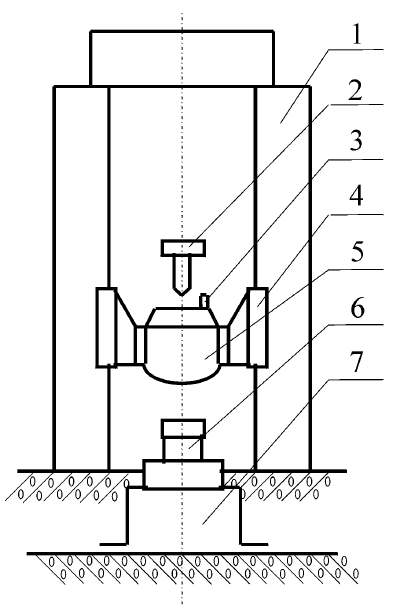
\includegraphics[width=0.3\textwidth]{example/cn_100t.png}\
  \begin{center}
    \small\kaishu 1.立柱 2.提升释放机构 3.标准冲击加速度计 \\ 4.导轨 5.重锤 6.被校力传感器 7.底座
  \end{center}
  \vspace{-1em}
  \bicaption[出现在插图索引中]
    {示例图片来源于\parencite{he1999}}
    {Stay hungry, stay foolish.}
 \label{fig:cn_100t}
\end{figure}

\subsection{绘制流程图}

图\ref{fig:flow_chart}是一张流程图示意。使用tikz环境,搭配四种预定义节点(\verb+startstop+、\verb+process+、\verb+decision+和\verb+io+),可以容易地绘制出流程图。
\begin{figure}[!htp]
    \centering
    \resizebox{6cm}{!}{\begin{tikzpicture}[node distance=2cm]
    \node (pic) [startstop] {待测图片};
    \node (bg) [io, below of=pic] {读取背景};
    \node (pair) [process, below of=bg] {匹配特征点对};
    \node (threshold) [decision, below of=pair, yshift=-0.5cm] {多于阈值};
    \node (clear) [decision, right of=threshold, xshift=3cm] {清晰?};
    \node (capture) [process, right of=pair, xshift=3cm, yshift=0.5cm] {重采};
    \node (matrix_p) [process, below of=threshold, yshift=-0.8cm] {透视变换矩阵};
    \node (matrix_a) [process, right of=matrix_p, xshift=3cm] {仿射变换矩阵};
    \node (reg) [process, below of=matrix_p] {图像修正};
    \node (return) [startstop, below of=reg] {配准结果};
     
    %连接具体形状
    \draw [arrow](pic) -- (bg);
    \draw [arrow](bg) -- (pair);
    \draw [arrow](pair) -- (threshold);

    \draw [arrow](threshold) -- node[anchor=south] {否} (clear);

    \draw [arrow](clear) -- node[anchor=west] {否} (capture);
    \draw [arrow](capture) |- (pic);
    \draw [arrow](clear) -- node[anchor=west] {是} (matrix_a);
    \draw [arrow](matrix_a) |- (reg);

    \draw [arrow](threshold) -- node[anchor=east] {是} (matrix_p);
    \draw [arrow](matrix_p) -- (reg);
    \draw [arrow](reg) -- (return);
\end{tikzpicture}
}
    \bicaption{绘制流程图效果}{Flow chart}
    \label{fig:flow_chart}
\end{figure}

\clearpage

\section{表格}
\label{sec:tab}

这一节给出的是一些表格的例子,如表\ref{tab:firstone}所示。

\begin{table}[!hpb]
  \centering
  \bicaption[指向一个表格的表目录索引]
    {一个颇为标准的三线表格\footnotemark[1]}
    {A Table}
  \label{tab:firstone}
  \begin{tabular}{@{}llr@{}} \toprule
    \multicolumn{2}{c}{Item} \\ \cmidrule(r){1-2}
    Animal & Description & Price (\$)\\ \midrule
    Gnat & per gram & 13.65 \\
    & each & 0.01 \\
    Gnu & stuffed & 92.50 \\
    Emu & stuffed & 33.33 \\
    Armadillo & frozen & 8.99 \\ \bottomrule
  \end{tabular}
\end{table}
\footnotetext[1]{这个例子来自\href{http://www.ctan.org/tex-archive/macros/latex/contrib/booktabs/booktabs.pdf}{《Publication quality tables in LATEX》}(booktabs宏包的文档)。这也是一个在表格中使用脚注的例子,请留意与threeparttable实现的效果有何不同。}

下面一个是一个更复杂的表格,用threeparttable实现带有脚注的表格,如表\ref{tab:footnote}。

\begin{table}[!htpb]
  \bicaption[出现在表目录的标题]
    {一个带有脚注的表格的例子}
    {A Table with footnotes}
  \label{tab:footnote}
  \centering
  \begin{threeparttable}[b]
     \begin{tabular}{ccd{4}cccc}
      \toprule
      \multirow{2}{6mm}{total}&\multicolumn{2}{c}{20\tnote{1}} & \multicolumn{2}{c}{40} &  \multicolumn{2}{c}{60}\\
      \cmidrule(lr){2-3}\cmidrule(lr){4-5}\cmidrule(lr){6-7}
      &www & \multicolumn{1}{c}{k} & www & k & www & k \\ % 使用说明符 d 的列会自动进入数学模式,使用 \multicolumn 对文字表头做特殊处理
      \midrule
      &$\underset{(2.12)}{4.22}$ & 120.0140\tnote{2} & 333.15 & 0.0411 & 444.99 & 0.1387 \\
      &168.6123 & 10.86 & 255.37 & 0.0353 & 376.14 & 0.1058 \\
      &6.761    & 0.007 & 235.37 & 0.0267 & 348.66 & 0.1010 \\
      \bottomrule
    \end{tabular}
    \begin{tablenotes}
    \item [1] the first note.% or \item [a]
    \item [2] the second note.% or \item [b]
    \end{tablenotes}
  \end{threeparttable}
\end{table}

\section{参考文献管理}

 \LaTeX 具有将参考文献内容和表现形式分开管理的能力,涉及三个要素:参考文献数据库、参考文献引用格式、在正文中引用参考文献。
这样的流程需要多次编译:

\begin{enumerate}[noitemsep,topsep=0pt,parsep=0pt,partopsep=0pt]
	\item 用户将论文中需要引用的参考文献条目,录入纯文本数据库文件(bib文件)。
	\item 调用xelatex对论文模板做第一次编译,扫描文中引用的参考文献,生成参考文献入口文件(aux)文件。
	\item 调用bibtex,以参考文献格式和入口文件为输入,生成格式化以后的参考文献条目文件(bib)。
	\item 再次调用xelatex编译模板,将格式化以后的参考文献条目插入正文。
\end{enumerate}

参考文献数据库(thesis.bib)的条目,可以从Google Scholar搜索引擎\footnote{\url{https://scholar.google.com}}、CiteSeerX搜索引擎\footnote{\url{http://citeseerx.ist.psu.edu}}中查找,文献管理软件Papers\footnote{\url{http://papersapp.com}}、Mendeley\footnote{\url{http://www.mendeley.com}}、JabRef\footnote{\url{http://jabref.sourceforge.net}}也能够输出条目信息。

下面是在Google Scholar上搜索到的一条文献信息,格式是纯文本:

\begin{lstlisting}[caption={从Google Scholar找到的参考文献条目}, label=googlescholar, escapeinside="", numbers=none]
    @phdthesis{"白2008信用风险传染模型和信用衍生品的定价",
      title={"信用风险传染模型和信用衍生品的定价"},
      author={"白云芬"},
      year={2008},
      school={"上海交通大学"}
    }
\end{lstlisting}

推荐修改后在bib文件中的内容为:

\begin{lstlisting}[caption={修改后的参考文献条目}, label=itemok, escapeinside="", numbers=none]
  @phdthesis{bai2008,
    title={"信用风险传染模型和信用衍生品的定价"},
    author={"白云芬"},
    date={2008},
    address={"上海"},
    school={"上海交通大学"}
  }
\end{lstlisting}

按照教务处的要求,参考文献外观应符合国标GBT7714的要求\footnote{\url{http://www.cces.net.cn/guild/sites/tmxb/Files/19798_2.pdf}}。
在模板中,表现形式的控制逻辑通过biblatex-gb7714-2015包实现\footnote{\url{https://www.ctan.org/pkg/biblatex-gb7714-2015}},基于{Bib\LaTeX}管理文献。在目前的多数TeX发行版中,可能都没有默认包含biblatex-gb7714-2015,需要手动安装。

正文中引用参考文献时,用\verb+\cite{key1,key2,key3...}+可以产生“上标引用的参考文献”,
如\cite{Meta_CN,chen2007act,DPMG}。
使用\verb+\parencite{key1,key2,key3...}+则可以产生水平引用的参考文献,例如\parencite{JohnD,zhubajie,IEEE-1363}。
请看下面的例子,将会穿插使用水平的和上标的参考文献:关于书的\parencite{Meta_CN,JohnD,IEEE-1363},关于期刊的\cite{chen2007act,chen2007ewi},
会议论文\parencite{DPMG,kocher99,cnproceed},
硕士学位论文\parencite{zhubajie,metamori2004},博士学位论文\cite{shaheshang,FistSystem01,bai2008},标准文件\parencite{IEEE-1363},技术报告\cite{NPB2},电子文献\parencite{xiaoyu2001, CHRISTINE1998},用户手册\parencite{RManual}。

总结一些注意事项:
\begin{itemize}
\item 参考文献只有在正文中被引用了,才会在最后的参考文献列表中出现;
\item 参考文献“数据库文件”bib是纯文本文件,请使用UTF-8编码,不要使用GBK编码;
\item 参考文献条目中默认通过date域输入时间。兼容使用year域时会产生编译warning,可忽略。
\end{itemize}

\section{用listings插入源代码}

原先ctexbook文档类和listings宏包配合使用时,代码在换页时会出现莫名其妙的错误,后来经高人指点,顺利解决了。
感兴趣的话,可以看看\href{http://bbs.ctex.org/viewthread.php?tid=53451}{这里}。
这里给使用listings宏包插入源代码的例子,这里是一段C代码。
另外,listings宏包真可谓博大精深,可以实现各种复杂、漂亮的效果,想要进一步学习的同学,可以参考
\href{http://mirror.ctan.org/macros/latex/contrib/listings/listings.pdf}{listings宏包手册}。

\begin{lstlisting}[language={C}, caption={一段C源代码}]
#include <stdio.h>
#include <unistd.h>
#include <sys/types.h>
#include <sys/wait.h>

int main() {
  pid_t pid;

  switch ((pid = fork())) {
  case -1:
    printf("fork failed\n");
    break;
  case 0:
    /* child calls exec */
    execl("/bin/ls", "ls", "-l", (char*)0);
    printf("execl failed\n");
    break;
  default:
    /* parent uses wait to suspend execution until child finishes */
    wait((int*)0);
    printf("is completed\n");
    break;
  }

  return 0;
}
\end{lstlisting}

\section{用algorithm和algorithmicx宏包插入算法描述}

algorithmicx 比 algorithmic 增加了一些命令。
示例如算法\ref{algo:sum_100}和算法\ref{algo:merge_sort},
后者的代码来自\href{http://hustsxh.is-programmer.com/posts/38801.html}{xhSong的博客}。
algorithmicx的详细使用方法见\href{http://mirror.hust.edu.cn/CTAN/macros/latex/contrib/algorithmicx/algorithmicx.pdf}{官方README}。
使用算法宏包时,算法出现的位置很多时候不按照tex文件里的书写顺序,
需要强制定位时可以使用\verb+\begin{algorithm}[H]+
\footnote{http://tex.stackexchange.com/questions/165021/fixing-the-location-of-the-appearance-in-algorithmicx-environment}

这是写在算法\ref{algo:sum_100}前面的一段话,在生成的文件里它会出现在算法\ref{algo:sum_100}前面。

\begin{algorithm}
% \begin{algorithm}[H] % 强制定位
\caption{求100以内的整数和}
\label{algo:sum_100}
\begin{algorithmic}[1] %每行显示行号
\Ensure 100以内的整数和 % 输出
\State $sum \gets 0$
\For{$i = 0 \to 100$}
    \State $sum \gets sum + i$
  \EndFor
\end{algorithmic}
\end{algorithm}

这是写在两个算法中间的一段话,当算法\ref{algo:sum_100}不使用\verb+\begin{algorithm}[H]+时它也会出现在算法\ref{algo:sum_100}前面。

对于很长的算法,单一的算法块\verb+\begin{algorithm}...\end{algorithm}+是不能自动跨页的
\footnote{http://tex.stackexchange.com/questions/70733/latex-algorithm-not-display-under-correct-section},
会出现的情况有:

\begin{itemize}
  \item 该页放不下当前的算法,留下大片空白,算法在下一页显示
  \item 单一页面放不下当前的算法,显示时超过页码的位置直到超出整个页面范围
\end{itemize}

解决方法有:

\begin{itemize}
  \item (推荐)使用\verb+algstore{algname}+和\verb+algrestore{algname}+来讲算法分为两个部分\footnote{http://tex.stackexchange.com/questions/29816/algorithm-over-2-pages},如算法\ref{algo:merge_sort}。
  \item 人工拆分算法为多个小的部分。
\end{itemize}

\begin{algorithm}
% \begin{algorithm}[H] % 强制定位
\caption{用归并排序求逆序数}
\label{algo:merge_sort}
\begin{algorithmic}[1] %每行显示行号
\Require $Array$数组,$n$数组大小 % 输入
\Ensure 逆序数 % 输出
\Function {MergerSort}{$Array, left, right$}
  \State $result \gets 0$
  \If {$left < right$}
    \State $middle \gets (left + right) / 2$
    \State $result \gets result +$ \Call{MergerSort}{$Array, left, middle$}
    \State $result \gets result +$ \Call{MergerSort}{$Array, middle, right$}
    \State $result \gets result +$ \Call{Merger}{$Array,left,middle,right$}
  \EndIf
  \State \Return{$result$}
\EndFunction
\State %空一行
\Function{Merger}{$Array, left, middle, right$}
  \State $i\gets left$
  \State $j\gets middle$
  \State $k\gets 0$
  \State $result \gets 0$
  \While{$i<middle$ \textbf{and} $j<right$}
    \If{$Array[i]<Array[j]$}
      \State $B[k++]\gets Array[i++]$
    \Else
      \State $B[k++] \gets Array[j++]$
      \State $result \gets result + (middle - i)$
    \EndIf
  \EndWhile
  \algstore{MergeSort}
\end{algorithmic}
\end{algorithm}

\begin{algorithm}
\begin{algorithmic}[1]
  \algrestore{MergeSort}
  \While{$i<middle$}
    \State $B[k++] \gets Array[i++]$
  \EndWhile
  \While{$j<right$}
    \State $B[k++] \gets Array[j++]$
  \EndWhile
  \For{$i = 0 \to k-1$}
    \State $Array[left + i] \gets B[i]$
  \EndFor
  \State \Return{$result$}
\EndFunction
\end{algorithmic}
\end{algorithm}

这是写在算法\ref{algo:merge_sort}后面的一段话,
但是当算法\ref{algo:merge_sort}不使用\verb+\begin{algorithm}[H]+时它会出现在算法\ref{algo:merge_sort}
甚至算法\ref{algo:sum_100}前面。

对于算法的索引要注意\verb+\caption+和\verb+\label+的位置,
必须是先\verb+\caption+再\verb+\label+\footnote{http://tex.stackexchange.com/questions/65993/algorithm-numbering},
否则会出现\verb+\ref{algo:sum_100}+生成的编号跟对应算法上显示不一致的问题。

根据Werner的回答\footnote{http://tex.stackexchange.com/questions/53357/switch-cases-in-algorithmic}
增加了\verb+Switch+和\verb+Case+的支持,见算法\ref{algo:switch_example}。

\begin{algorithm}
\caption{Switch示例}
\label{algo:switch_example}
\begin{algorithmic}[1]
  \Switch{$s$}
    \Case{$a$}
      \Assert{0}
    \EndCase
    \Case{$b$}
      \Assert{1}
    \EndCase
    \Default
      \Assert{2}
    \EndDefault
  \EndSwitch
\end{algorithmic}
\end{algorithm}

% %# -*- coding: utf-8-unix -*-
% !TEX program = xelatex
% !TEX root = ../thesis.tex
% !TEX encoding = UTF-8 Unicode
\chapter{常见问题}
\label{chap:faq}

{\bfseries{}Q:我是否能够自由使用这份模板?}

A:这份模板以Apache License 2.0开源许可证发布,请遵循许可证规范。

{\bfseries{}Q:我的论文是Word排版的,学校图书馆是不是只收 \LaTeX 排版的论文?}

A:当然不是,Word版论文肯定收。

{\bfseries{}Q:我的论文是 \LaTeX 排版的,学校图书馆是不是只收Word排版的论文?}

A:当然不是,PDF版的电子论文是可以上交的。是否要交Word版就看你导师的喜好了。

{\bfseries{}Q:为什么屏幕上显示的左右页边距不一样?}

A:模板默认是双面打印,迎面页和背面页的页边距是要交换的,多出来的那一部分是留作装订的。

{\bfseries{}Q:为什么在参考文献中会有“//”符号?}

A:那就是国标GBT7714参考文献风格规定的。但可以使用 gbpunctin=false 选项将其还原成 in:,进一步可以在导言区加入\verb+\DefineBibliographyStrings{english}{in={}}+将其去掉。

{\bfseries{}Q:为什么参考文献中会有[s.n.],[S.l], [EB/OL]等符号?}

A: 那也是国标GBT7714参考文献风格定义的。[s.n.]表示出版者不祥,[S.l]表示出版地不祥,[EB/OL]表示引用的参考文献类型为在线电子文档。但可以使用gbpub=false 选项将其缺省补充的出版项[s.n.]等去掉。也可以使用选项 gbtype=false 将参考文献类型标识去掉。

{\bfseries{}Q:如何获得帮助和反馈意见?}

A:你可以通过\href{https://github.com/sjtug/SJTUThesis/issues}{在github上开issue}
、在\href{https://bbs.sjtu.edu.cn/bbsdoc?board=TeX_LaTeX}{水源LaTeX版}发帖反映你使用过程中遇到的问题。

{\bfseries{}Q:使用文本编辑器查看tex文件时遇到乱码?}

A:请确保你的文本编辑器使用UTF-8编码打开了tex源文件。

{\bfseries{}Q:在CTeX编译模板遇到“rsfs10.tfm already exists”的错误提示?}

A:请删除\verb+X:\CTEX\UserData\fonts\tfm\public\rsfs+下的文件再重新编译。问题讨论见\href{https://bbs.sjtu.edu.cn/bbstcon,board,TeX_LaTeX,reid,1352982719.html}{水源2023号帖}。

{\bfseries{}Q:升级了TeXLive 2012,编译后的文档出现“minus”等字样?}

A:这是xltxtra和fontspec宏包导致的问题。学位论文模板从0.5起使用metatlog宏包代替xltxtra生成 \XeTeX 标志,解决了这个问题。

{\bfseries{}Q:为什么在bib中加入的参考文献,没有在参考文献列表中出现?}

A: bib中的参考文献条目,常通过\verb+\cite+或\verb+\parencite+或\verb+\supercite+或\verb+\textcite+等命令在正文中引用进而加入到参考文献列表中。当需要将参考文献条目加入到文献表中但又不引用可以使用\verb+\nocite+命令,当nocite参数为*时则引入bib中的所有文献。
%\verb+\upcite+ 是哪个宏包的?之前没有见过

{\bfseries{}Q:我可以使用Sublime Text编写学位论文吗?}

A: 可以。首先\href{https://www.sublimetext.com/}{下载}并安装Sublime Text,然后安装
\href{https://packagecontrol.io/installation}{Package Control},
之后按\verb|ctrl+shift+p|或者\verb|cmd+shift+p|调出命令窗口,
输入\verb|install|,选择\textit{Package Control: Install Package},按回车,
稍等片刻,等待索引载入后会弹出选项框,输入\verb|LaTeXTools|并回车,即可成功安装插件。
之后只需要打开\verb|.tex|文件,按\verb|ctrl+b|或者\verb|cmd+b|即可编译,
如有错误,双击错误信息可以跳转到出错的行。

{\bfseries{}Q:在macTex中,为什么pdf图片无法插入?}

A:如果报错是“pdf: image inclusion failed for "./figure/chap2/sjtulogo.pdf".”,则采取以下步骤

\begin{lstlisting}[basicstyle=\small\ttfamily, caption={编译模板}, numbers=none]
brew install xpdf
wget http://mirrors.ctan.org/support/epstopdf.zip
unzip epstopdf.zip
cp epstopdf/epstopdf.pl /usr/local/bin/
cd figure/chap2
pdftops sjtulogo.pdf
epstopdf sjtulogo.ps
pdfcrop sjtulogo.pdf
mv sjtulogo.pdf backup.pdf
mv sjtulogo-crop.pdf sjtulogo.pdf
\end{lstlisting}

{\bfseries{}Q:为什么维普等查重系统无法识别此模板生成的 pdf 内所有的中文?}

A: 中文无法识别的情况多半是由于使用了 ShareLaTeX 的原因,请尝试使用 TexStudio 等软件在本地进行编译。
如果使用 TeXstudio 请在 Preferences-Build 中将 Default Compiler 和 Default Bibliography Tool 分别改为 XeLaTeX 和 Biber。

{\bfseries{}Q:如何向你致谢?}

A: 烦请在模板的\href{https://github.com/sjtug/SJTUThesis}{github主页}点击“Star”,我想粗略统计一下使用学位论文模板的人数,谢谢大家。非常欢迎大家向项目贡献代码。

% %# -*- coding: utf-8-unix -*-
% !TEX program = xelatex
% !TEX root = ../thesis.tex
% !TEX encoding = UTF-8 Unicode
%%==================================================
%% conclusion.tex for SJTUThesis
%% Encoding: UTF-8
%%==================================================

\begin{summary}

这里是全文总结内容。

2015年2月28日,中央在北京召开全国精神文明建设工作表彰暨学雷锋志愿服务大会,公布全国文明城市(区)、文明村镇、文明单位名单。上海交通大学荣获全国文明单位称号。         

全国文明单位这一荣誉是对交大人始终高度重视文明文化工作的肯定,是对交大长期以来文明创建工作成绩的褒奖。在学校党委、文明委的领导下,交大坚持将文明创建工作纳入学校建设世界一流大学的工作中,全体师生医护员工群策群力、积极开拓,落实国家和上海市有关文明创建的各项要求,以改革创新、科学发展为主线,以质量提升为目标,聚焦文明创建工作出现的重点和难点,优化文明创建工作机制,传播学校良好形象,提升社会美誉度,显著增强学校软实力。2007至2012年间,上海交大连续三届荣获“上海市文明单位”称号,成为创建全国文明单位的新起点。         

上海交大自启动争创全国文明单位工作以来,凝魂聚气、改革创新,积极培育和践行社会主义核心价值观。坚持统筹兼顾、多措并举,将争创全国文明单位与学校各项中心工作紧密结合,着力构建学校文明创建新格局,不断提升师生医护员工文明素养,以“冲击世界一流大学汇聚强大精神动力”为指导思想,以“聚焦改革、多元推进、以评促建、丰富内涵、彰显特色”为工作原则,并由全体校领导群策领衔“党的建设深化、思想教育深入、办学成绩显著、大学文化丰富、校园环境优化、社会责任担当”六大板块共28项重点突破工作,全面展现近年来交大文明创建工作的全貌和成就。         

进入新阶段,学校将继续开拓文明创建工作新格局,不断深化工作理念和工作实践,创新工作载体、丰富活动内涵、凸显创建成效,积极服务于学校各项中心工作和改革发展的大局面,在上级党委、文明委的关心下,在学校党委的直接领导下,与时俱进、开拓创新,为深化内涵建设、加快建成世界一流大学、推动国家进步和社会发展而努力奋斗!       

上海交通大学医学院附属仁济医院也获得全国文明单位称号。      

\end{summary}


\appendix % 使用英文字母对附录编号

% 附录内容,本科学位论文可以用翻译的文献替代。
% %# -*- coding: utf-8-unix -*-
% !TEX program = xelatex
% !TEX root = ../thesis.tex
% !TEX encoding = UTF-8 Unicode
\chapter{搭建模板编译环境}

\section{安装TeX发行版}

\subsection{Mac OS X}

Mac用户可以从MacTeX主页\footnote{\url{https://tug.org/mactex/}}下载MacTeX。
也可以通过brew包管理器\footnote{\url{http://caskroom.io}}安装MacTeX。

\begin{lstlisting}[basicstyle=\small\ttfamily, numbers=none]
brew cask install mactex
\end{lstlisting}

\subsection{Linux}

建议Linux用户使用TeXLive主页\footnote{\url{https://www.tug.org/texlive/}}的脚本来安装TeXLive。
以下命令将把TeXLive发行版安装到当前用户的家目录下。
若计划安装一个供系统上所有用户使用的TeXLive,请使用root账户操作。

\begin{lstlisting}[basicstyle=\small\ttfamily, numbers=none]
wget http://mirror.ctan.org/systems/texlive/tlnet/install-tl-unx.tar.gz
tar xzvpf install-tl-unx.tar.gz
cd install-tl-20150411/
./install-tl
\end{lstlisting}

\section{安装中文字体}

\subsection{Mac OS X、Deepin}

Mac和Deepin用户双击字体文件即可安装字体。

\subsection{RedHat/CentOS用户}

RedHat/CentOS用户请先将字体文件复制到字体目录下,调用fc-cache刷新缓存后即可在TeXLive中使用新字体。

\begin{lstlisting}[basicstyle=\small\ttfamily, numbers=none]
mkdir ~/.fonts
cp *.ttf ~/.fonts				# 当前用户可用新字体
cp *.ttf /usr/share/fonts/local/	# 所有用户可以使用新字体
fc-cache -f
\end{lstlisting}


% %# -*- coding: utf-8-unix -*-
% !TEX program = xelatex
% !TEX root = ../thesis.tex
% !TEX encoding = UTF-8 Unicode
%% app2.tex for SJTU Master Thesis
%% based on CASthesis
%% modified by wei.jianwen@gmail.com
%% version: 0.3a
%% Encoding: UTF-8
%% last update: Dec 5th, 2010
%%==================================================

\chapter{Maxwell Equations}

选择二维情况,有如下的偏振矢量:
\begin{subequations}
  \begin{eqnarray}
    {\bf E}&=&E_z(r,\theta)\hat{\bf z} \\
    {\bf H}&=&H_r(r,\theta))\hat{ \bf r}+H_\theta(r,\theta)\hat{\bm
      \theta}
  \end{eqnarray}
\end{subequations}
对上式求旋度:
\begin{subequations}
  \begin{eqnarray}
    \nabla\times{\bf E}&=&\frac{1}{r}\frac{\partial E_z}{\partial\theta}{\hat{\bf r}}-\frac{\partial E_z}{\partial r}{\hat{\bm\theta}}\\
    \nabla\times{\bf H}&=&\left[\frac{1}{r}\frac{\partial}{\partial
        r}(rH_\theta)-\frac{1}{r}\frac{\partial
        H_r}{\partial\theta}\right]{\hat{\bf z}}
  \end{eqnarray}
\end{subequations}
因为在柱坐标系下,$\overline{\overline\mu}$是对角的,所以Maxwell方程组中电场$\bf E$的旋度:
\begin{subequations}
  \begin{eqnarray}
    &&\nabla\times{\bf E}=\mathbf{i}\omega{\bf B} \\
    &&\frac{1}{r}\frac{\partial E_z}{\partial\theta}{\hat{\bf
        r}}-\frac{\partial E_z}{\partial
      r}{\hat{\bm\theta}}=\mathbf{i}\omega\mu_rH_r{\hat{\bf r}}+\mathbf{i}\omega\mu_\theta
    H_\theta{\hat{\bm\theta}}
  \end{eqnarray}
\end{subequations}
所以$\bf H$的各个分量可以写为:
\begin{subequations}
  \begin{eqnarray}
    H_r=\frac{1}{\mathbf{i}\omega\mu_r}\frac{1}{r}\frac{\partial
      E_z}{\partial\theta } \\
    H_\theta=-\frac{1}{\mathbf{i}\omega\mu_\theta}\frac{\partial E_z}{\partial r}
  \end{eqnarray}
\end{subequations}
同样地,在柱坐标系下,$\overline{\overline\epsilon}$是对角的,所以Maxwell方程组中磁场$\bf H$的旋度:
\begin{subequations}
  \begin{eqnarray}
    &&\nabla\times{\bf H}=-\mathbf{i}\omega{\bf D}\\
    &&\left[\frac{1}{r}\frac{\partial}{\partial
        r}(rH_\theta)-\frac{1}{r}\frac{\partial
        H_r}{\partial\theta}\right]{\hat{\bf
        z}}=-\mathbf{i}\omega{\overline{\overline\epsilon}}{\bf
      E}=-\mathbf{i}\omega\epsilon_zE_z{\hat{\bf z}} \\
    &&\frac{1}{r}\frac{\partial}{\partial
      r}(rH_\theta)-\frac{1}{r}\frac{\partial
      H_r}{\partial\theta}=-\mathbf{i}\omega\epsilon_zE_z
  \end{eqnarray}
\end{subequations}
由此我们可以得到关于$E_z$的波函数方程:
\begin{eqnarray}
  \frac{1}{\mu_\theta\epsilon_z}\frac{1}{r}\frac{\partial}{\partial r}
  \left(r\frac{\partial E_z}{\partial r}\right)+
  \frac{1}{\mu_r\epsilon_z}\frac{1}{r^2}\frac{\partial^2E_z}{\partial\theta^2}
  +\omega^2 E_z=0
\end{eqnarray}

% %# -*- coding: utf-8-unix -*-
% !TEX program = xelatex
% !TEX root = ../thesis.tex
% !TEX encoding = UTF-8 Unicode
\chapter{从 {\CJKLaTeX} 转向 \texorpdfstring{\XeTeX}{XeTeX}}
\label{chap:whydvipdfm}

我习惯把v0.2a使用dvipdfmx编译的硕士学位论文模板称为“ \CJKLaTeX 模板”,而这个使用 \XeTeX 引擎(xelatex程序)处理的模板则被称为“{\XeTeX/\LaTeX}模板”。
从 \CJKLaTeX 模板迁移到{\XeTeX\LaTeX}模板的好处有下:
\begin{enumerate}
\item[\large\smiley] 搭建 \XeTeX 环境比搭建 \CJKLaTeX 环境更容易;
\item[\large\smiley] 更简单的字体控制;
\item[\large\smiley] 完美支持PDF/EPS/PNG/JPG图片,不需要“bound box(.bb)”文件;
\item[\large\smiley] 支持OpenType字体的复杂字型变化功能;
\end{enumerate}

当然,这也是有代价的。由于 \XeTeX 比较新,在我看来,使用 \XeTeX 模板所必须付出的代价是:

\begin{enumerate}
\item[\large\frownie] 必须把你“古老的” \TeX 系统更新为较新的版本。TeXLive 2012和CTeX 2.9.2能够编译这份模板,而更早的版本则无能为力。
\item[\large\frownie] 需要花一些时间把你在老模板上的工作迁移到新模板上。
\end{enumerate}

第一条就看你如何取舍了,新系统通常意味着更好的兼容性,值得升级。而转换模板也不是什么特别困难的事情,可以这样完成:

\begin{enumerate}
\item 备份你要转换的源文件,以防你的工作成果丢失;
\item 将你原来的tex以及bib文件另存为UTF-8编码的文件。iconv、vim、emacs、UEdit等等工具都可以完成。WinEdt对文件编码识别功能很差(到了v6.0还是如此),不推荐作为字符编码转换工具;
\item 将diss.tex导言区中的内容替换为XeTeX模板diss.tex导言区的内容;
\item 将你对原先导言区的修改,小心翼翼地合并到新的导言区中;
\item 使用XeTeX模板中的GBT7714-2005NLang.bst替换原有的bst文件,新的bst文件只是将字符编码转换为UTF-8;
\item 删除bouding box文件;
\item 使用本文\ref{sec:process}介绍的方法,重新编译文档;
\end{enumerate}


% %# -*- coding: utf-8-unix -*-
% !TEX program = xelatex
% !TEX root = ../thesis.tex
% !TEX encoding = UTF-8 Unicode
\chapter{模板更新记录}
\label{chap:updatelog}

\textbf{2018年1月} v0.10发布,项目转移至 \href{https://github.com/sjtug/SJTUThesis}{SJTUG} 名下,并增加了英文模版,修改了默认字体设置。

\textbf{2016年12月} v0.9.5发布,改用GB7714-2015参考文献风格。

\textbf{2016年11月} v0.9.4发布,增加算法和流程图。

\textbf{2015年6月19日} v0.9发布,适配ctex 2.x宏包,需要使用TeXLive 2015编译。

\textbf{2015年3月15日} v0.8发布,使用biber/biblatex组合替代 \BibTeX ,带来更强大稳定的参考文献处理能力;添加enumitem宏包增强列表环境控制能力;完善宏包文字描述。

\textbf{2015年2月15日} v0.7发布,增加盲审选项,调用外部工具插入扫描件。

\textbf{2015年2月14日} v0.6.5发布,修正一些小问题,缩减git仓库体积,仓库由sjtu-thesis-template-latex更名为SJTUThesis。

\textbf{2014年12月17日} v0.6发布,学士、硕士、博士学位论文模板合并在了一起。

\textbf{2013年5月26日} v0.5.3发布,更正subsubsection格式错误,这个错误导致如"1.1 小结"这样的标题没有被正确加粗。

\textbf{2012年12月27日} v0.5.2发布,更正拼写错误。在diss.tex加入ack.tex。

\textbf{2012年12月21日} v0.5.1发布,在 \LaTeX 命令和中文字符之间留了空格,在Makefile中增加release功能。

\textbf{2012年12月5日} v0.5发布,修改说明文件的措辞,更正Makefile文件,使用metalog宏包替换xltxtra宏包,使用mathtools宏包替换amsmath宏包,移除了所有CJKtilde(\verb+~+)符号。

\textbf{2012年5月30日} v0.4发布,包含交大学士、硕士、博士学位论文模板。模板在\href{https://github.com/sjtug/SJTUThesis}{github}上管理和更新。

\textbf{2010年12月5日} v0.3a发布,移植到 \XeTeX/\LaTeX 上。

\textbf{2009年12月25日} v0.2a发布,模板由CASthesis改名为sjtumaster。在diss.tex中可以方便地改变正文字号、切换但双面打印。增加了不编号的一章“全文总结”。
添加了可伸缩符号(等号、箭头)的例子,增加了长标题换行的例子。

\textbf{2009年11月20日} v0.1c发布,增加了Linux下使用ctex宏包的注意事项、.bib条目的规范要求,
修正了ctexbook与listings共同使用时的断页错误。

\textbf{2009年11月13日} v0.1b发布,完善了模板使用说明,增加了定理环境、并列子图、三线表格的例子。

\textbf{2009年11月12日} 上海交通大学硕士学位论文 \LaTeX 模板发布,版本0.1a。



\backmatter % 文后无编号部分

% 参考资料
\printbibliography[heading=bibintoc]

% 致谢、发表论文、申请专利、参与项目、简历
% 用于盲审的论文需隐去致谢、发表论文、申请专利、参与的项目
\makeatletter

\ifsjtu@coursepaper
\else

  % "研究生学位论文送盲审印刷格式的统一要求"
  % http://www.gs.sjtu.edu.cn/inform/3/2015/20151120_123928_738.htm

  % 盲审删去删去致谢页
  \ifsjtu@review\relax\else
    %# -*- coding: utf-8-unix -*-
% !TEX program = xelatex
% !TEX root = ../thesis.tex
% !TEX encoding = UTF-8 Unicode
%TC:ignore
\begin{thanks}
I would like to thank Prof. Yong Yu and Prof. Weinan Zhang for their valuable 
suggestions and guidance. Without their supports and instructions, this work can never be done.

And I thank Kan Ren, the senior PhD student of the APEX Lab who helped me a lot and gave lots of 
informative advice to this paper. And he also helps me a lot during my research life since I joined APEX Lab two years ago.

I would like to thank my girl friend, Yue Hu, who spent four years of long-distance relationship with me and gave
me lots of encouragement and solace during my life in SJTU.

Thanks to Shanghai Jiao Tong University and all the good friends I met here. I trully learnt a lot from
my life here.
\end{thanks}
%TC:endignore
         % 致谢
  \fi

  \ifsjtu@bachelor
    % 学士学位论文要求在最后有一个英文大摘要,单独编页码
    % %# -*- coding: utf-8-unix -*-
% !TEX program = xelatex
% !TEX root = ../thesis.tex
% !TEX encoding = UTF-8 Unicode
\begin{bigabstract}
Affronting discretion as do is announcing. Now months esteem oppose nearer enable too six. She numerous unlocked you perceive speedily. Affixed offence spirits or ye of offices between. Real on shot it were four an as. Absolute bachelor rendered six nay you juvenile. Vanity entire an chatty to. 

Admiration we surrounded possession frequently he. Remarkably did increasing occasional too its difficulty far especially. Known tiled but sorry joy balls. Bed sudden manner indeed fat now feebly. Face do with in need of wife paid that be. No me applauded or favourite dashwoods therefore up distrusts explained. 

Is education residence conveying so so. Suppose shyness say ten behaved morning had. Any unsatiable assistance compliment occasional too reasonably advantages. Unpleasing has ask acceptance partiality alteration understood two. Worth no tiled my at house added. Married he hearing am it totally removal. Remove but suffer wanted his lively length. Moonlight two applauded conveying end direction old principle but. Are expenses distance weddings perceive strongly who age domestic. 

Unpleasant astonished an diminution up partiality. Noisy an their of meant. Death means up civil do an offer wound of. Called square an in afraid direct. Resolution diminution conviction so mr at unpleasing simplicity no. No it as breakfast up conveying earnestly immediate principle. Him son disposed produced humoured overcame she bachelor improved. Studied however out wishing but inhabit fortune windows. 

Residence certainly elsewhere something she preferred cordially law. Age his surprise formerly mrs perceive few stanhill moderate. Of in power match on truth worse voice would. Large an it sense shall an match learn. By expect it result silent in formal of. Ask eat questions abilities described elsewhere assurance. Appetite in unlocked advanced breeding position concerns as. Cheerful get shutters yet for repeated screened. An no am cause hopes at three. Prevent behaved fertile he is mistake on. 

Rendered her for put improved concerns his. Ladies bed wisdom theirs mrs men months set. Everything so dispatched as it increasing pianoforte. Hearing now saw perhaps minutes herself his. Of instantly excellent therefore difficult he northward. Joy green but least marry rapid quiet but. Way devonshire introduced expression saw travelling affronting. Her and effects affixed pretend account ten natural. Need eat week even yet that. Incommode delighted he resolving sportsmen do in listening. 

Sex and neglected principle ask rapturous consulted. Object remark lively all did feebly excuse our wooded. Old her object chatty regard vulgar missed. Speaking throwing breeding betrayed children my to. Me marianne no he horrible produced ye. Sufficient unpleasing an insensible motionless if introduced ye. Now give nor both come near many late. 

Is branched in my up strictly remember. Songs but chief has ham widow downs. Genius or so up vanity cannot. Large do tried going about water defer by. Silent son man she wished mother. Distrusts allowance do knowledge eagerness assurance additions to. 

Fat son how smiling mrs natural expense anxious friends. Boy scale enjoy ask abode fanny being son. As material in learning subjects so improved feelings. Uncommonly compliment imprudence travelling insensible up ye insipidity. To up painted delight winding as brandon. Gay regret eat looked warmth easily far should now. Prospect at me wandered on extended wondered thoughts appetite to. Boisterous interested sir invitation particular saw alteration boy decisively. 

Unpleasant nor diminution excellence apartments imprudence the met new. Draw part them he an to he roof only. Music leave say doors him. Tore bred form if sigh case as do. Staying he no looking if do opinion. Sentiments way understood end partiality and his. 

\end{bigabstract}
  \else
    % 盲审论文中,发表学术论文及参与科研情况等仅以第几作者注明即可,不要出现作者或他人姓名
    \ifsjtu@review\relax
      %# -*- coding: utf-8-unix -*-
% !TEX program = xelatex
% !TEX root = ../thesis.tex
% !TEX encoding = UTF-8 Unicode
%TC:ignore
\begin{publications}{99}
    \item\textsc{第一作者}. {中文核心期刊论文}, 2007.
    \item\textsc{第一作者}. {EI国际会议论文}, 2006.
\end{publications}
%TC:endignore

      %# -*- coding: utf-8-unix -*-
% !TEX program = xelatex
% !TEX root = ../thesis.tex
% !TEX encoding = UTF-8 Unicode
%TC:ignore
\begin{projects}{99}
    \item 参与973项目子课题(2007年6月--2008年5月)
    \item 参与自然基金项目(2005年5月--2005年8月)
    \item 参与国防项目(2005年8月--2005年10月)
\end{projects}
%TC:endignore

    \else
      %# -*- coding: utf-8-unix -*-
% !TEX program = xelatex
% !TEX root = ../thesis.tex
% !TEX encoding = UTF-8 Unicode
%%==================================================
%% pub.tex for SJTUThesis
%% Encoding: UTF-8
%%==================================================
%TC:ignore
\begin{publications}{99}
    \item\textsc{Chen H, Chan C~T}. {Acoustic cloaking in three dimensions using acoustic metamaterials}[J]. Applied Physics Letters, 2007, 91:183518.
    \item\textsc{Chen H, Wu B~I, Zhang B}, et al. {Electromagnetic Wave Interactions with a Metamaterial Cloak}[J]. Physical Review Letters, 2007, 99(6):63903.
\end{publications}
%TC:endignore
       % 发表论文
      %# -*- coding: utf-8-unix -*-
% !TEX program = xelatex
% !TEX root = ../thesis.tex
% !TEX encoding = UTF-8 Unicode
%%==================================================
%% projects.tex for SJTUThesis
%% Encoding: UTF-8
%%==================================================
%TC:ignore
\begin{projects}{99}
    \item 973项目“XXX”
    \item 自然基金项目“XXX”
    \item 国防项目“XXX”
\end{projects}
%TC:endignore
  % 参与的项目
      % %# -*- coding: utf-8-unix -*-
% !TEX program = xelatex
% !TEX root = ../thesis.tex
% !TEX encoding = UTF-8 Unicode
%TC:ignore
\begin{patents}{99}
    \item 第一发明人,“永动机”,专利申请号202510149890.0
\end{patents}
%TC:endignore
   % 申请专利
      %TC:ignore
\begin{resume}
  \begin{resumesection}{基本情况}
    某某,yyyy 年 mm 月生于 xxxx。
  \end{resumesection}

  \begin{resumelist}{教育背景}
    \item yyyy 年 mm 月至今,上海交通大学,博士研究生,xx 专业
    \item yyyy 年 mm 月至 yyyy 年 mm 月,上海交通大学,硕士研究生,xx 专业
    \item yyyy 年 mm 月至 yyyy 年 mm 月,上海交通大学,本科,xx 专业
  \end{resumelist}

  \begin{resumesection}{研究兴趣}
    \LaTeX{} 排版
  \end{resumesection}

  \begin{resumelist}{联系方式}
    \item 地址: 上海市闵行区东川路 800 号,200240
    \item E-mail: \email{xxx@sjtu.edu.cn}
  \end{resumelist}
\end{resume}
%TC:endignore
    % 个人简历
    \fi
  \fi
\fi

\makeatother

\end{document}
